\documentclass[12pt]{article}

\usepackage{Preamble}

%! Author = sbbfti
%! Date = 10/06/2020

\newacronym{ADF}{ADF test}{Augmented Dickey-Fuller test}
\newacronym{KPSS}{KPSS test}{Kwiatkowski-Phillips-Schmidt-Shin test}
\newacronym{ACF}{ACF}{AutoCorrelation function}
\newacronym{PACF}{PACF}{Partial AutoCorrelation function}


\newacronym{ti}{$T_{i}$}{indoor air temperature, $^{\circ}$C}


\title{Assignment \#1}				% Title
\author{Saeed Kazemi}				% Author
\date{\today}						% Date

\makeatletter
\let\theauthor\@author
\let\thedate\@date
\let\thetitle\@title
\makeatother
\begin{document}

%%%%%%%%%%%%%%%%%%%%%%%%%%%%%%%%%%%%%%%%%%%%%%%%%%%%%%%%%%%%%%%%%


\begin{titlepage}
	\centering
    \vspace*{0.4 cm}
    
\includegraphics[scale = 0.5]{figures/unb.jpg}\\[1.0 cm]	% University Logo
    \textsc{\LARGE \newline\newline University of New Brunswick}\\[1.8 cm]	% University Name
	\textsc{\Large Time Series Analysis\\(EE 6563)}\\[0.5 cm]				% Course Code
	\rule{\linewidth}{0.2 mm} \\[0.4 cm]
	{ \huge \bfseries \thetitle}\\
	\rule{\linewidth}{0.2 mm} \\[1.5 cm]
	
	\begin{minipage}{0.5\textwidth}
		\begin{flushleft} \large
			\emph{Professor:}\\
			Erik Scheme\\
            Electrical and Computer Engineering\\
			\end{flushleft}
			\end{minipage}~
			\begin{minipage}{0.5\textwidth}
            
			\begin{flushright} \large
			\emph{Author:} \\
			Saeed Kazemi\\ (3713280)\\

		\end{flushright}
        
	\end{minipage}\\[1 cm]
	
	
    \thedate
    
    
    
	
\end{titlepage}

%%%%%%%%%%%%%%%%%%%%%%%%%%%%%%%%%%%%%%%%%%%%%%%%%%%%%%%%%%%%%%%%%



%\tableofcontents
\pagebreak

%%%%%%%%%%%%%%%%%%%%%%%%%%%%%%%%%%%%%%%%%%%%%%%%%%%%%%%%%%%%%%%%%
%================================================================
\begin{enumerate}

\item \textbf{Download the following datasets:}
\begin{enumerate}
\item \textbf{Minimum Daily Temperatures Dataset}:This dataset describes the minimum daily temperatures over 10 years (1981-1990) in the city Melbourne, Australia. The units are in degrees Celsius and there are 3650 observations. The source of the data is credited as the Australian Bureau of Meteorology  (\href{https://raw.githubusercontent.com/jbrownlee/Datasets/master/daily-min-temperatures.csv}{ Source}).
\item \textbf{Monthly Sunspot Dataset}:This dataset describes a monthly count of the number of observed sunspots for just over 230 years (1749-1983). The units are a count and there are 2,820 observations. The source of the dataset is credited to Andrews \& Herzberg (1985) (\href{https://raw.githubusercontent.com/jbrownlee/Datasets/master/monthly-sunspots.csv}{ Source}).
\end{enumerate}

%%%%%%%%%%%%%%%%%%%%%%%%%%%%%%%%%%%%%%%%%%%%%%%%%%%%%%%%%%%%%%%%%
%%%%%%%%%%%%%%%%%%%%%%%% Question 1 %%%%%%%%%%%%%%%%%%%%%%%%%%%%%
%%%%%%%%%%%%%%%%%%%%%%%%%%%%%%%%%%%%%%%%%%%%%%%%%%%%%%%%%%%%%%%%%
\newpage
\item \textbf{For each dataset, visualize the raw signals, identify any trends, seasonality, and/or other components, and try to remove them. Remember that you are not limited to the tools shown in the tutorial and should explore the various concepts discussed in class. You do not need to explain the theory behind the approaches, but you should provide justification for their use, and discussion of their results.}


\textit{Figures \ref{fig:Ass1_D1_raw_signal} and \ref{fig:Ass1_D2_raw_signal} indicate the raw signal of both data sets. Likewise, figure \ref{fig:Ass1_D1_raw_signal_1986} to  \ref{fig:Ass1_D2_raw_signal_1990} illustrate a short period in two datasets. }

\begin{figure}[H]
    \centering
    \begin{minipage}[b]{1\textwidth}
        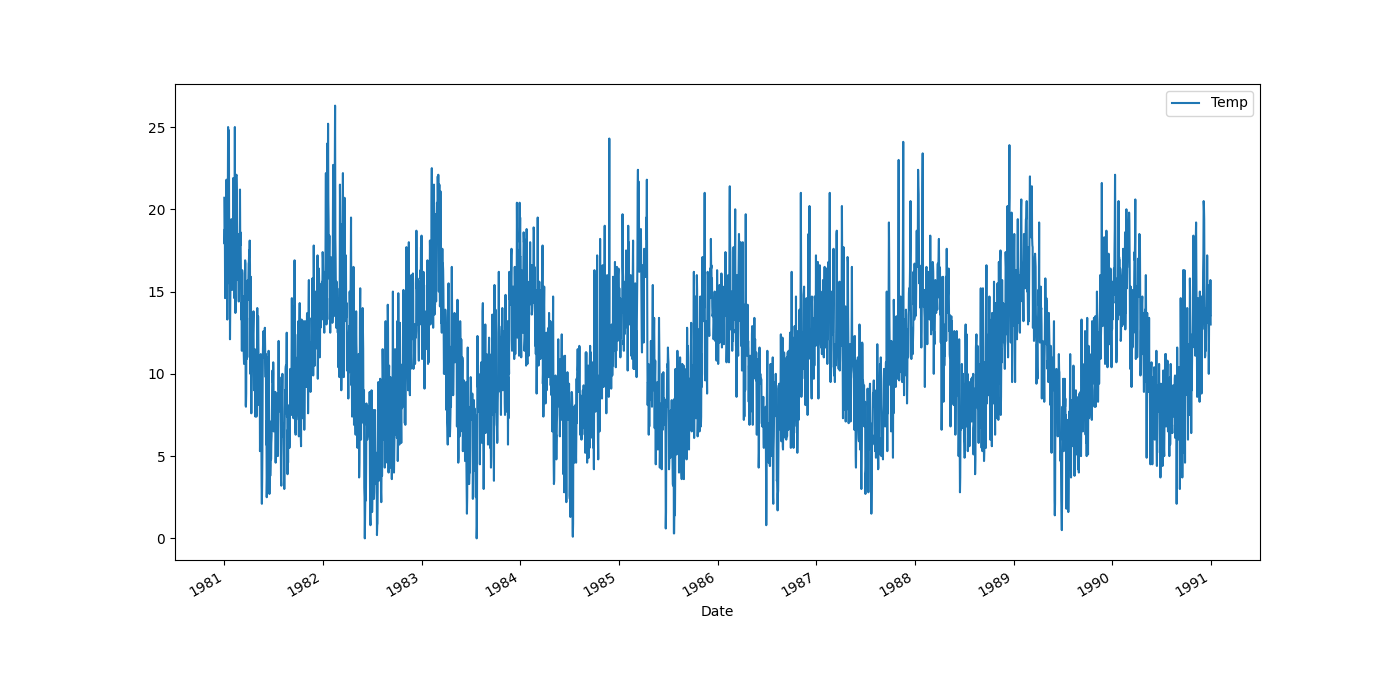
\includegraphics[width=\textwidth]{figures/Ass1/Ass1_D1_raw_signal.png}
    \end{minipage}
    \caption{The raw signal of the first dataset.}
    \label{fig:Ass1_D1_raw_signal}
\end{figure}

\begin{figure}[H]
    \centering
    \begin{minipage}[b]{1\textwidth}
        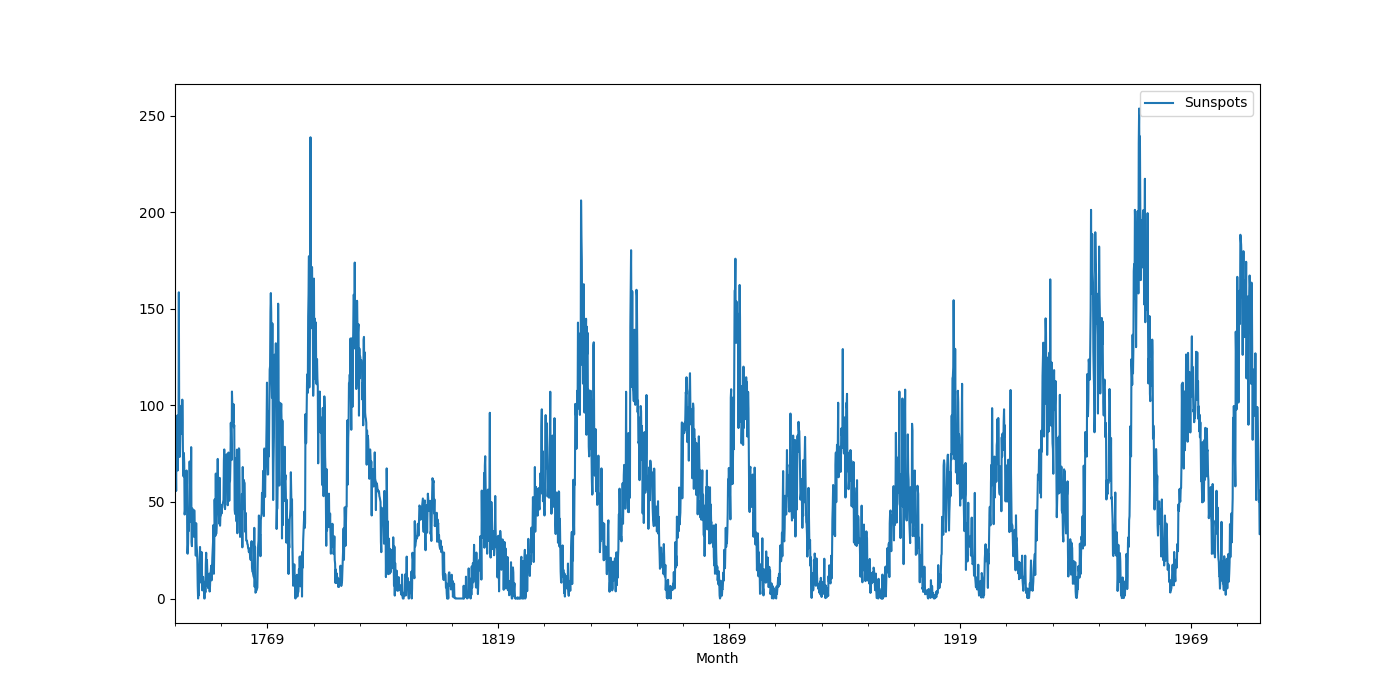
\includegraphics[width=\textwidth]{figures/Ass1/Ass1_D2_raw_signal.png}
    \end{minipage}
    \caption{The raw signal of the second dataset.}
    \label{fig:Ass1_D2_raw_signal}
\end{figure}

\begin{figure}[H]
    \centering
    \begin{minipage}[b]{1\textwidth}
        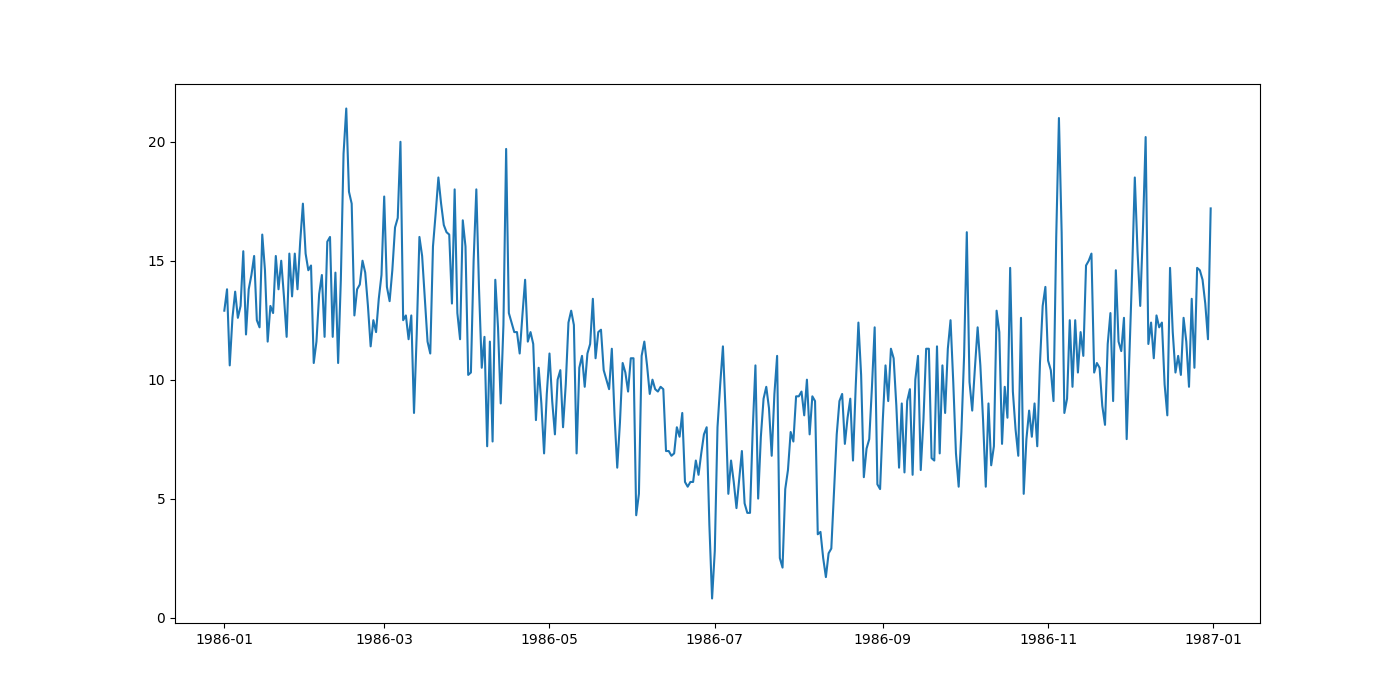
\includegraphics[width=\textwidth]{figures/Ass1/Ass1_D1_raw_signal_1986.png}
    \end{minipage}
    \caption{Visualizing a short period of the first dataset.}
    \label{fig:Ass1_D1_raw_signal_1986}
\end{figure}


\begin{figure}[H]
    \centering
    \begin{minipage}[b]{1\textwidth}
        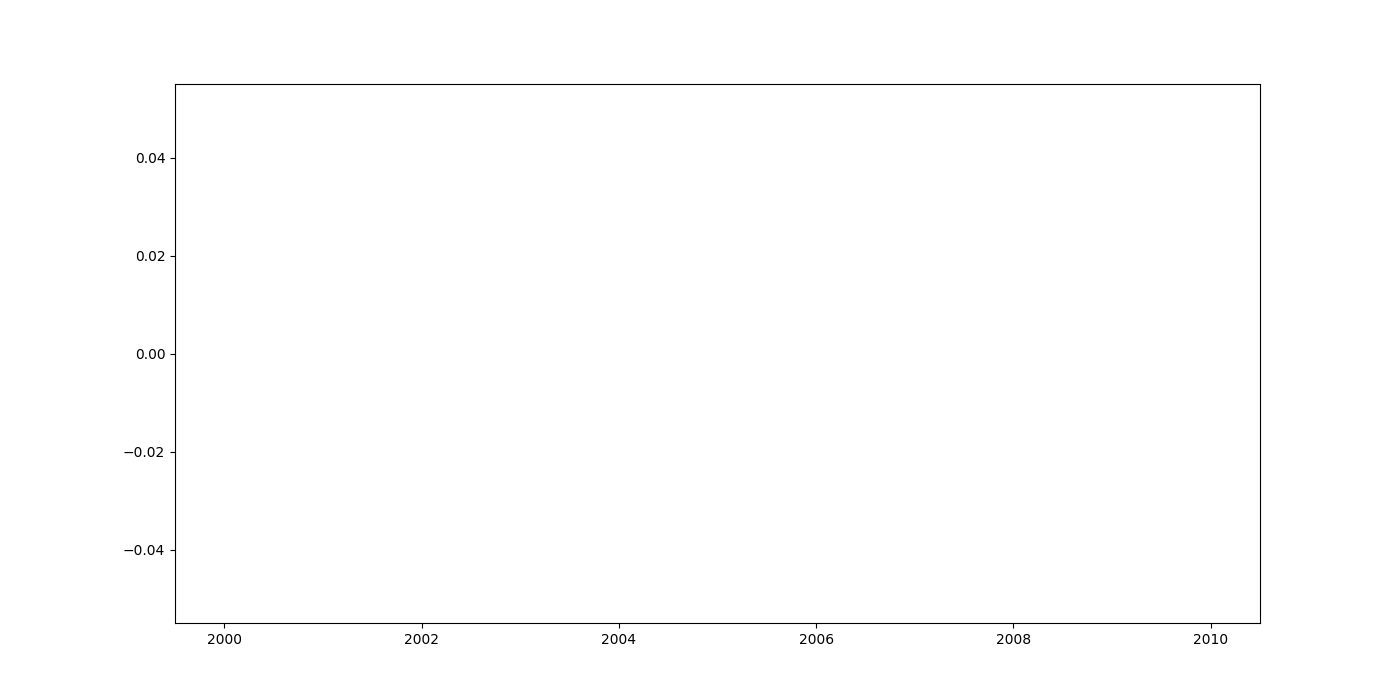
\includegraphics[width=\textwidth]{figures/Ass1/Ass1_D2_raw_signal_1990.png}
    \end{minipage}
    \caption{Visualizing a short period of the second dataset.}
    \label{fig:Ass1_D2_raw_signal_1990}
\end{figure}

\textit{For intuition, Table \ref{tab:Ass1_D1_raw_signal} to  \ref{tab:Ass1_D2_raw_signal_summary_statistics} show the top raw of two datasets along with the descriptive statistics of two time-series datasets.}


\begin{table}[H]
 \centering
\caption{The first five rows of the raw signal in the first dataset.}
\label{tab:Ass1_D1_raw_signal}
\begin{tabular}{lr}
\toprule
{} &  Temp \\
Date       &       \\
\midrule
1981-01-01 &  20.7 \\
1981-01-02 &  17.9 \\
1981-01-03 &  18.8 \\
1981-01-04 &  14.6 \\
1981-01-05 &  15.8 \\
1981-01-06 &  15.8 \\
1981-01-07 &  15.8 \\
\bottomrule
\end{tabular}

\end{table}

\begin{table}[H]
 \centering
\caption{The descriptive statistics of the first dataset.}
\label{tab:Ass1_D1_raw_signal_summary_statistics}
\begin{tabular}{lr}
\toprule
{} &         Temp \\
\midrule
count &  3650.000000 \\
mean  &    11.177753 \\
std   &     4.071837 \\
min   &     0.000000 \\
25\%   &     8.300000 \\
50\%   &    11.000000 \\
75\%   &    14.000000 \\
max   &    26.300000 \\
\bottomrule
\end{tabular}

\end{table}

\begin{table}[H]
 \centering
\caption{The first five rows of the raw signal in the second dataset.}
\label{tab:Ass1_D2_raw_signal}
\begin{tabular}{lr}
\toprule
{} &  Sunspots \\
Month      &           \\
\midrule
1749-01-01 &      58.0 \\
1749-02-01 &      62.6 \\
1749-03-01 &      70.0 \\
1749-04-01 &      55.7 \\
1749-05-01 &      85.0 \\
\bottomrule
\end{tabular}

\end{table}

\begin{table}[H]
 \centering
\caption{The descriptive statistics of the second dataset.} \label{tab:Ass1_D2_raw_signal_summary_statistics}
\begin{tabular}{lr}
\toprule
{} &     Sunspots \\
\midrule
count &  2820.000000 \\
mean  &    51.265957 \\
std   &    43.448971 \\
min   &     0.000000 \\
25\%   &    15.700000 \\
50\%   &    42.000000 \\
75\%   &    74.925000 \\
max   &   253.800000 \\
\bottomrule
\end{tabular}

\end{table}






\textit{For decomposing the time series, the below methods used:}
    \begin{enumerate}
    \item \textit{Seasonal\_decompose (Figure
        \ref{fig:Ass1_D1_seasonal_decompose} and \ref{fig:Ass1_D2_seasonal_decompose})}
        
    \item \textit{STL (Figure
        \ref{fig:Ass1_D1_STL} and \ref{fig:Ass1_D2_STL})}
        
    \item \textit{Linear Regression method (Figure
        \ref{fig:Ass1_D1_LinearRegression_diff} and \ref{fig:Ass1_D2_LinearRegression_diff})}
        
    \item \textit{Difference method (Figure
        \ref{fig:Ass1_D1_one_diff} and \ref{fig:Ass1_D2_one_diff})}
        
    \item \textit{Fitting a polynomial (Figure
        \ref{fig:Ass1_D1_fiting_polynomial} and \ref{fig:Ass1_D2_fiting_polynomial})}
        
    \item \textit{Moving Average window (Figure
        \ref{fig:Ass1_D1_Moving_Avrage} and \ref{fig:Ass1_D2_Moving_Avrage})}

    \end{enumerate}

\textit{\newline \newline Some mentioned methods used only for extracting only one type of component (trend or seasonality), while others like STL 
and Seasonal\_decompose provided all three parts. Table \ref{tab:Ass1_comparing_methods} compares these methods together.}

\textit{Also, there are two models for the reconstruction of time series, Additive and Multiplicative Model. In this assignment, the additive model was only used because the multiplicative model is not appropriate for zero and negative values.}

\begin{table}[H]
\centering
\caption{Comparing the implemented methods.}
\label{tab:Ass1_comparing_methods}
\begin{tabular}{@{}lccc@{}}
\toprule
                    & \begin{tabular}[c]{@{}c@{}}Trend \\ component\end{tabular} & \begin{tabular}[c]{@{}c@{}}Seasonal \\ component\end{tabular} & \begin{tabular}[c]{@{}c@{}}Residual \\ component\end{tabular} \\ \midrule
Seasonal\_decompose & \checkmark                                  & \checkmark                                     & \checkmark                                     \\ \midrule
STL                 & \checkmark                                  & \checkmark                                     & \checkmark                                     \\ \midrule
Linear Regression   & \checkmark                                  & -                                                             & -                                                             \\ \midrule
Difference          & -                                                          & \checkmark                                     & -                                                             \\ \midrule
Moving average      & \checkmark                                  & -                                                             & -                                                             \\ \bottomrule
\end{tabular}

\end{table}


\textit{For finding the seasonal component, we need to find the period of the time series. For doing this, the resampling method was used to smooth the plots of two datasets. Figures \ref{fig:Ass1_D1_resample} and \ref{fig:Ass1_D2_resample} indicate the smooth version of the two datasets. }

\begin{figure}[H]
    \centering
    \begin{minipage}[b]{1\textwidth}
        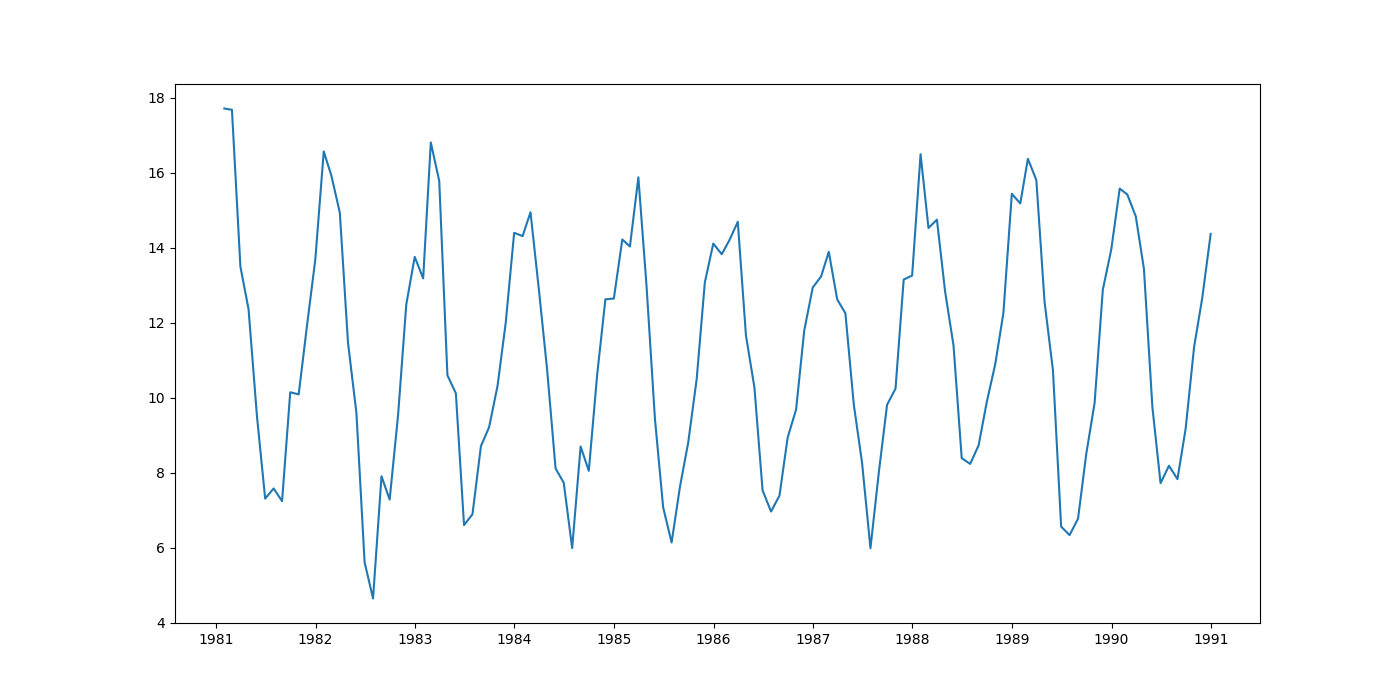
\includegraphics[width=\textwidth]{figures/Ass1/Ass1_D1_resample.png}
    \end{minipage}
    \caption{Resampling plot of the first dataset. The period of this dataset is 365 samples/cycle. }
    \label{fig:Ass1_D1_resample}
\end{figure}

\begin{figure}[H]
    \centering
    \begin{minipage}[b]{1\textwidth}
        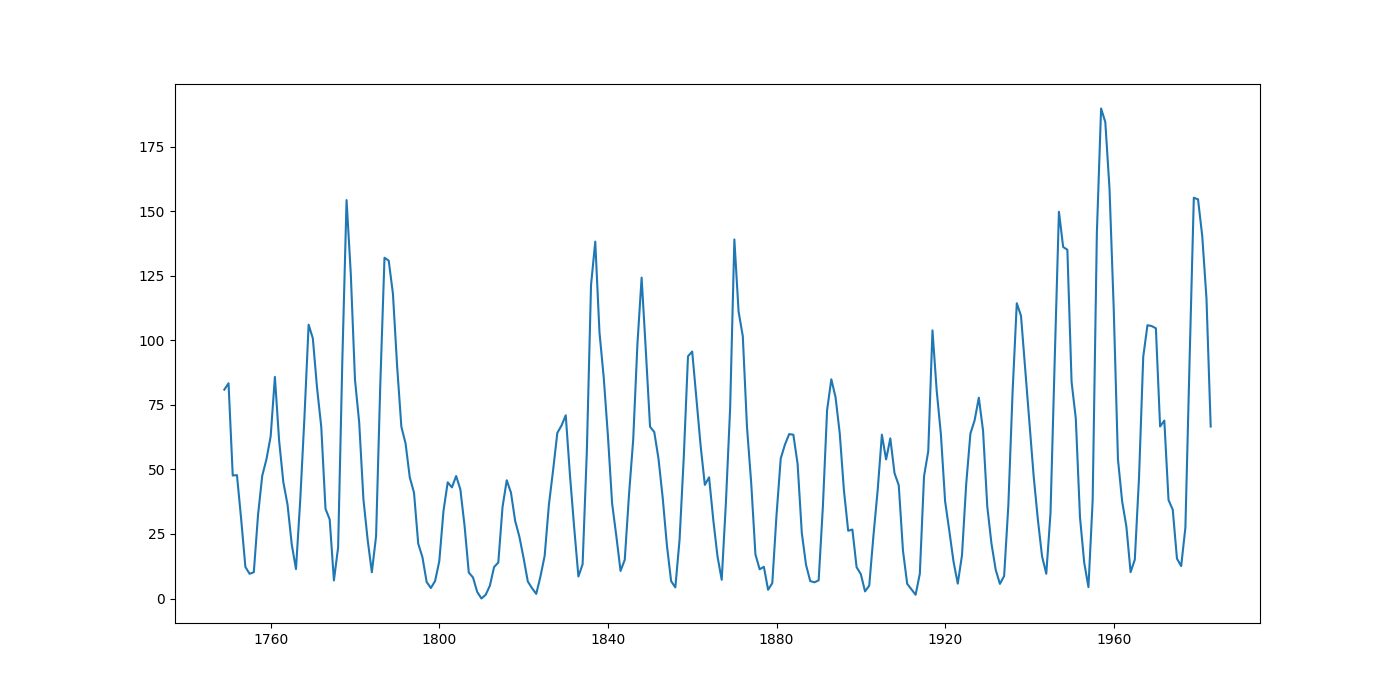
\includegraphics[width=\textwidth]{figures/Ass1/Ass1_D2_resample.png}
    \end{minipage}
    \caption{Resampling plot of the second dataset. The period of this dataset is 130 samples/cycle.}
    \label{fig:Ass1_D2_resample}
\end{figure}


\textit{Furthermore, the period of the time-series data can calculate by \gls{ACF} (figures \ref{fig:Ass1_D1_PACF_ACF_series} and \ref{fig:Ass1_D2_PACF_ACF_series}). This plot has an oscillation, indicative of a seasonal series and the peaks occurred at each period. }

\begin{figure}[H]
    \centering
    \begin{minipage}[b]{1\textwidth}
        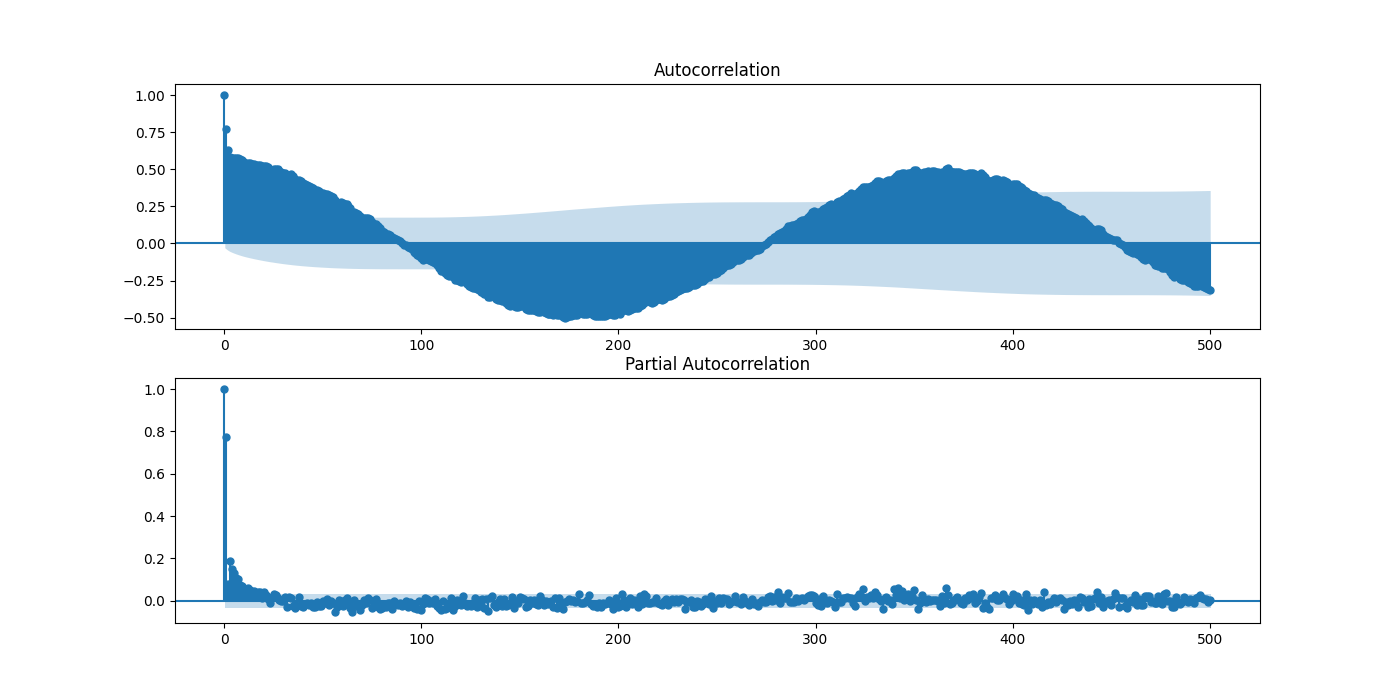
\includegraphics[width=\textwidth]{figures/Ass1/Ass1_D1_PACF_ACF_series.png}
    \end{minipage}
    \caption{The \gls{ACF} and \gls{PACF} of the first dataset. The peaks occur at the lag of 365 that means the period is 365 samples/cycle.}
    \label{fig:Ass1_D1_PACF_ACF_series}
\end{figure}

\begin{figure}[H]
    \centering
    \begin{minipage}[b]{1\textwidth}
        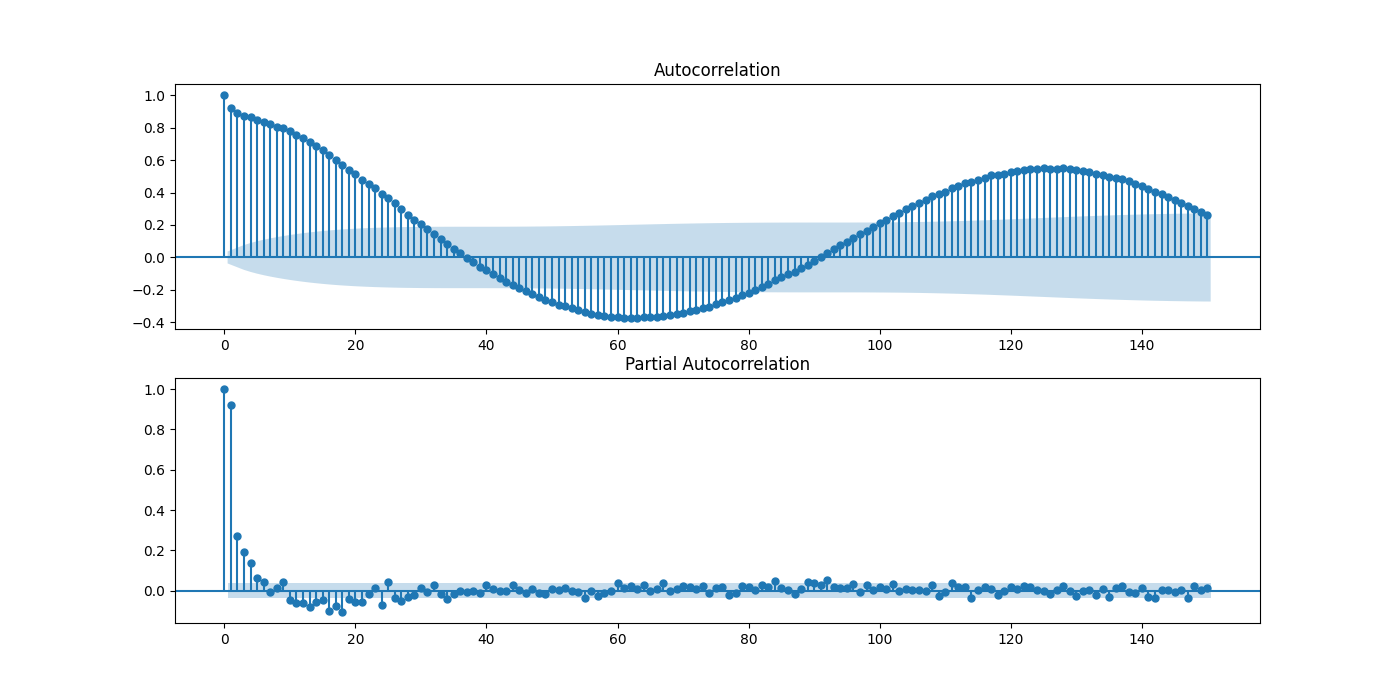
\includegraphics[width=\textwidth]{figures/Ass1/Ass1_D2_PACF_ACF_series.png}
    \end{minipage}
    \caption{The \gls{ACF} and \gls{PACF} of the second dataset. The peaks occur at the lag of 130 that means the period is 130 samples/cycle.}
    \label{fig:Ass1_D2_PACF_ACF_series}
\end{figure}


\begin{figure}[H]
    \centering
    \begin{minipage}[b]{1\textwidth}
        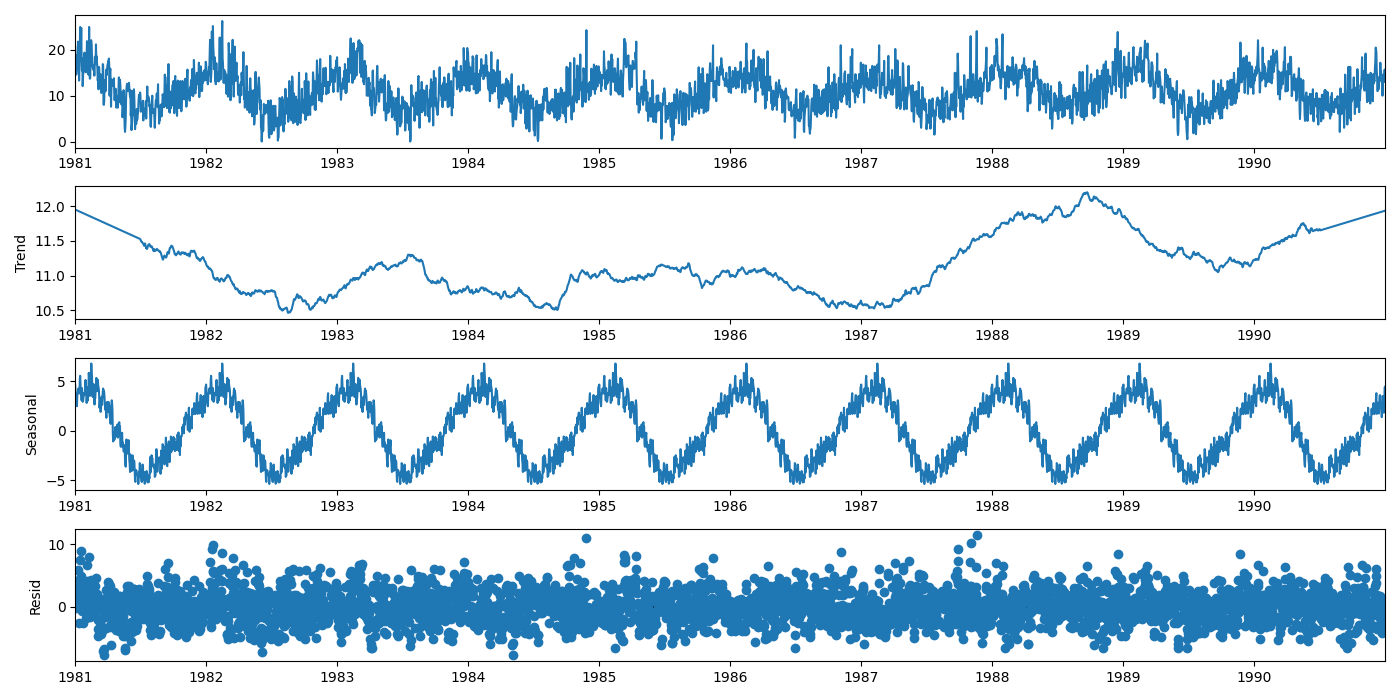
\includegraphics[width=\textwidth]{figures/Ass1/Ass1_D1_seasonal_decompose.png}
    \end{minipage}
    \caption{Decomposition of the first dataset by seasonal\_decompose method}
    \label{fig:Ass1_D1_seasonal_decompose}
\end{figure}

\begin{figure}[H]
    \centering
    \begin{minipage}[b]{1\textwidth}
        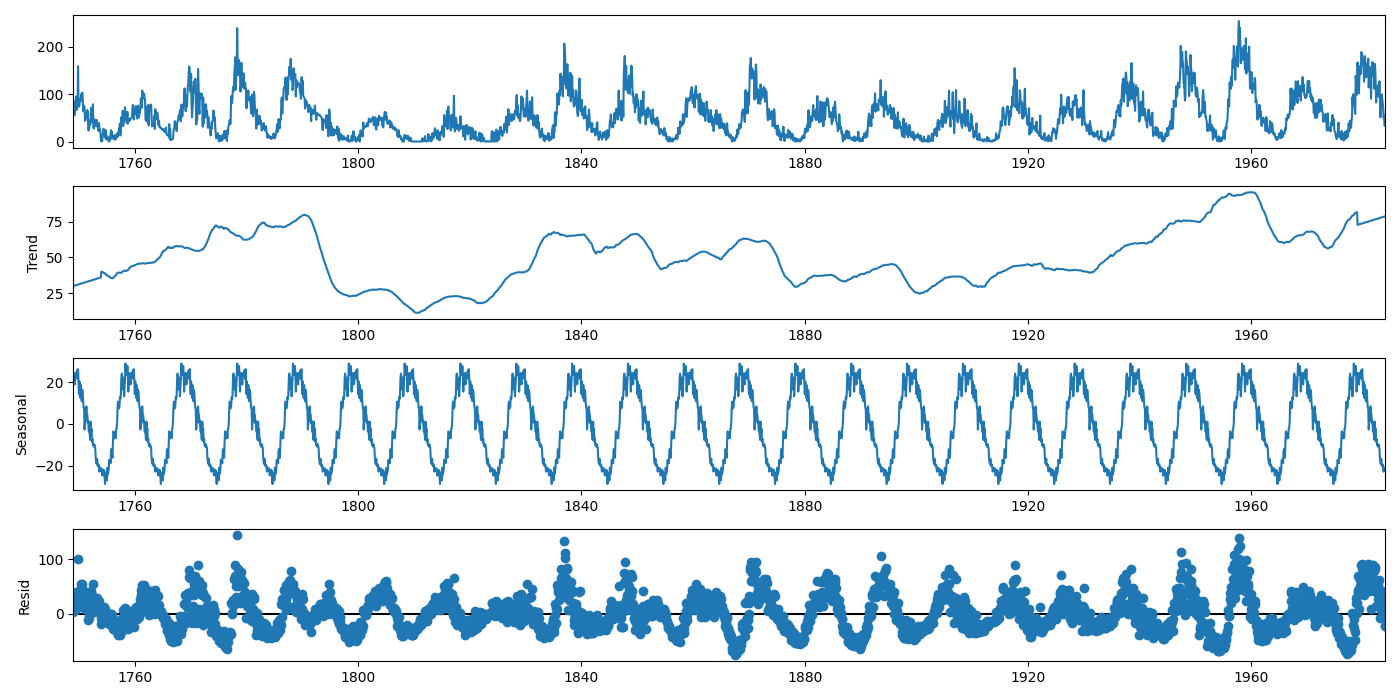
\includegraphics[width=\textwidth]{figures/Ass1/Ass1_D2_seasonal_decompose.png}
    \end{minipage}
    \caption{Decomposition of the second dataset by seasonal\_decompose method}
    \label{fig:Ass1_D2_seasonal_decompose}
\end{figure}

\begin{figure}[H]
    \centering
    \begin{minipage}[b]{1\textwidth}
        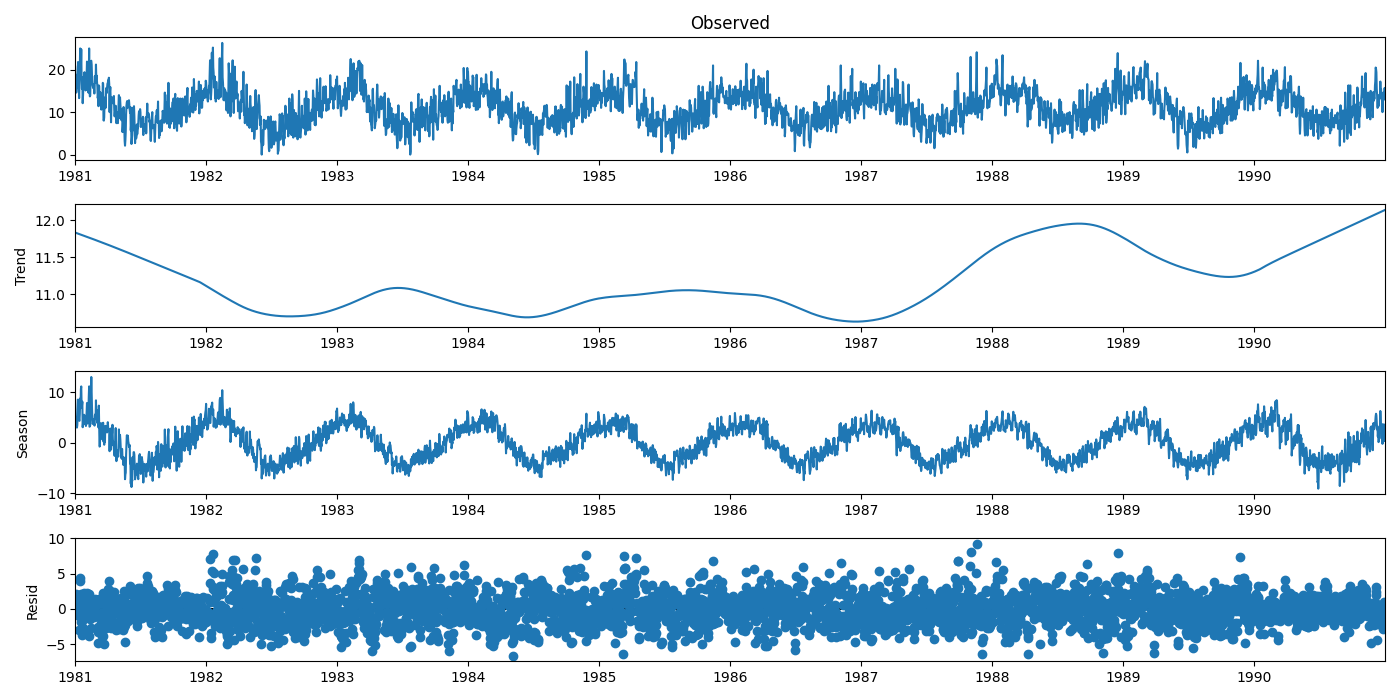
\includegraphics[width=\textwidth]{figures/Ass1/Ass1_D1_STL.png}
    \end{minipage}
    \caption{Decomposition of the first dataset by STL method}
    \label{fig:Ass1_D1_STL}
\end{figure}

\begin{figure}[H]
    \centering
    \begin{minipage}[b]{1\textwidth}
        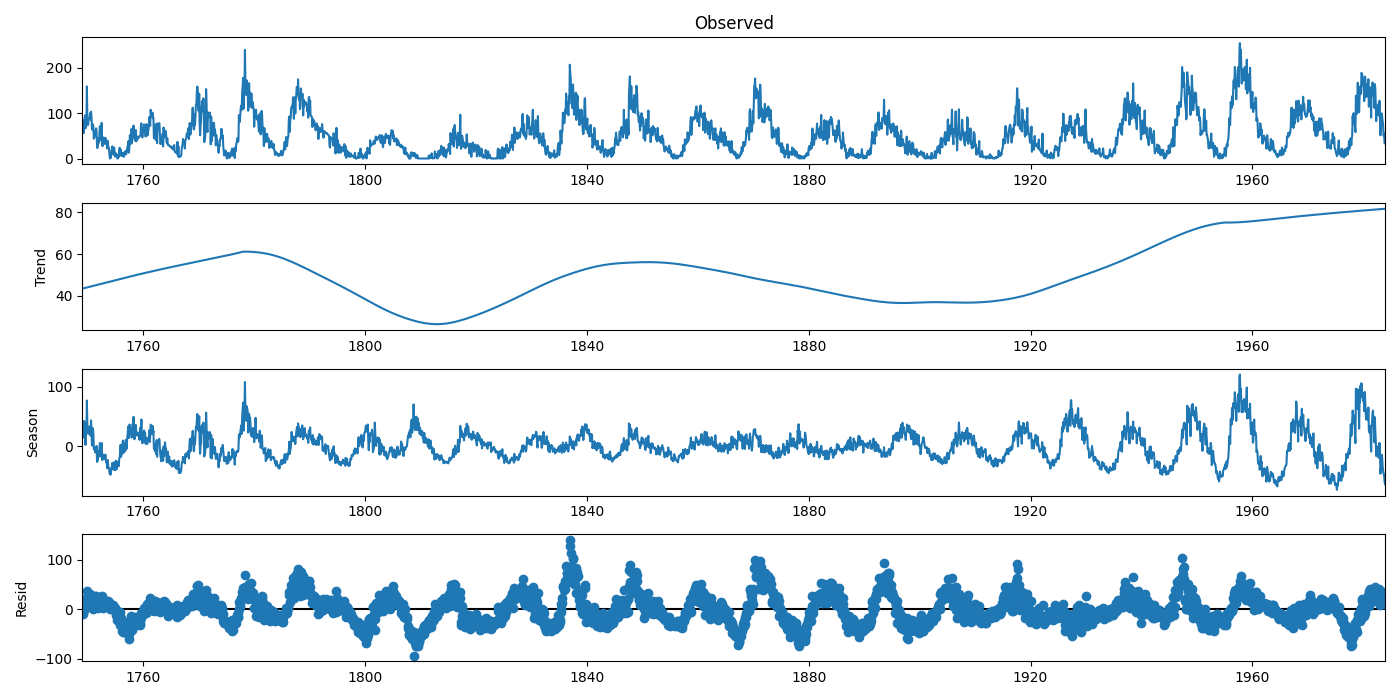
\includegraphics[width=\textwidth]{figures/Ass1/Ass1_D2_STL.png}
    \end{minipage}
    \caption{Decomposition of the second dataset by STL method}
    \label{fig:Ass1_D2_STL}
\end{figure}

\begin{figure}[H]
    \centering
    \begin{minipage}[b]{1\textwidth}
        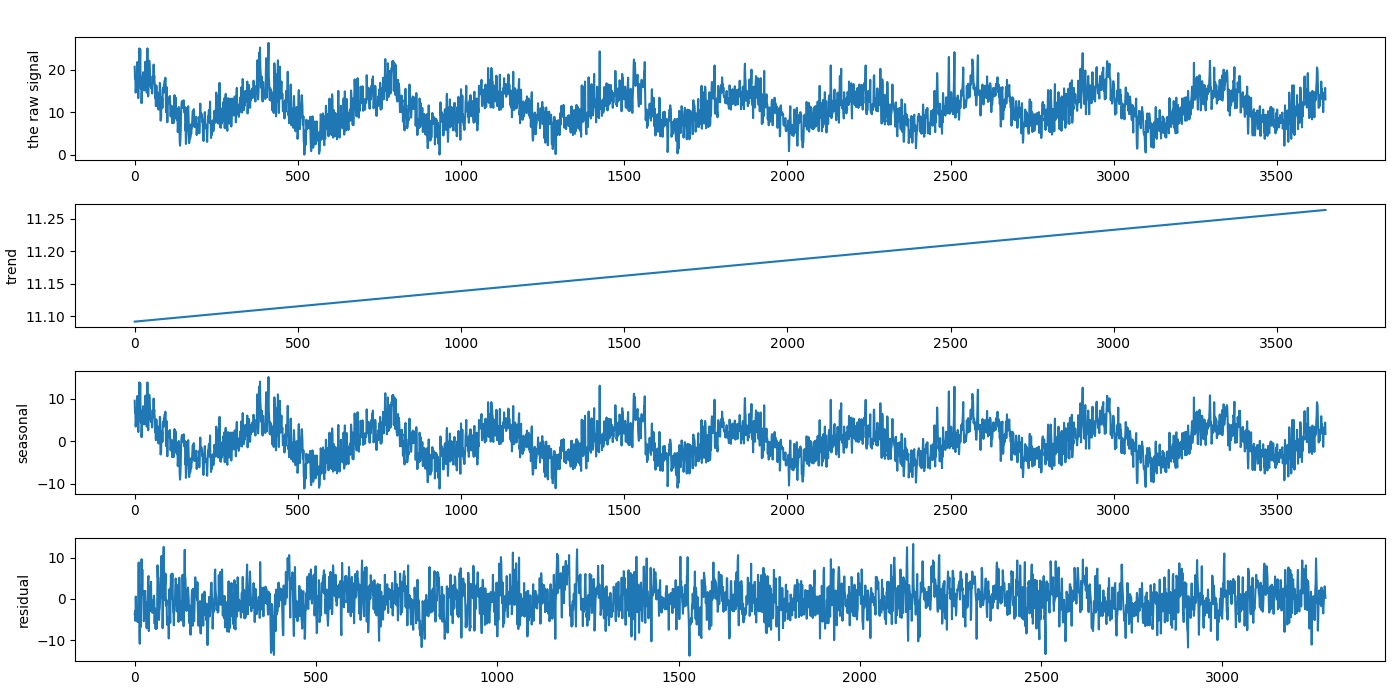
\includegraphics[width=\textwidth]{figures/Ass1/Ass1_D1_LinearRegression_diff.png}
    \end{minipage}
    \caption{Decomposition of the first dataset by Linear Regression and difference method.}
    \label{fig:Ass1_D1_LinearRegression_diff}
\end{figure}

\begin{figure}[H]
    \centering
    \begin{minipage}[b]{1\textwidth}
        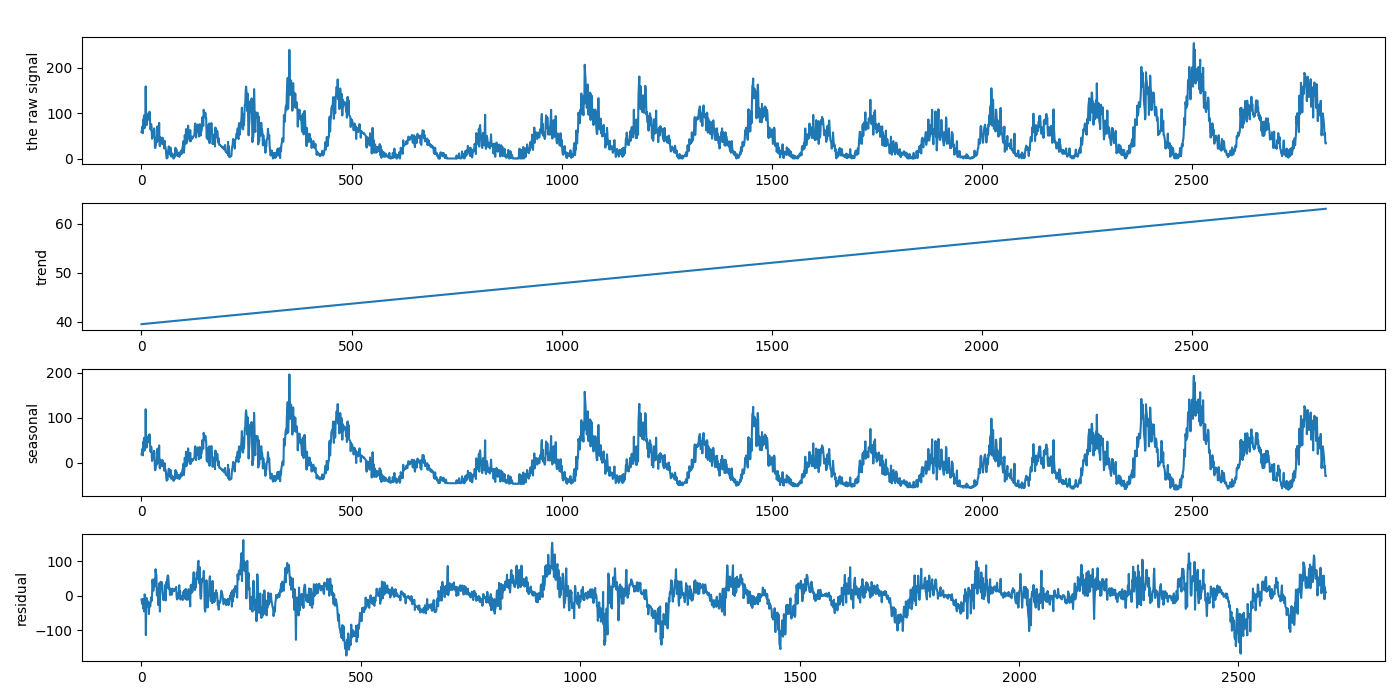
\includegraphics[width=\textwidth]{figures/Ass1/Ass1_D2_LinearRegression_diff.png}
    \end{minipage}
    \caption{Decomposition of the second dataset by Linear Regression and difference method.}
    \label{fig:Ass1_D2_LinearRegression_diff}
\end{figure}

\begin{figure}[H]
    \centering
    \begin{minipage}[b]{1\textwidth}
        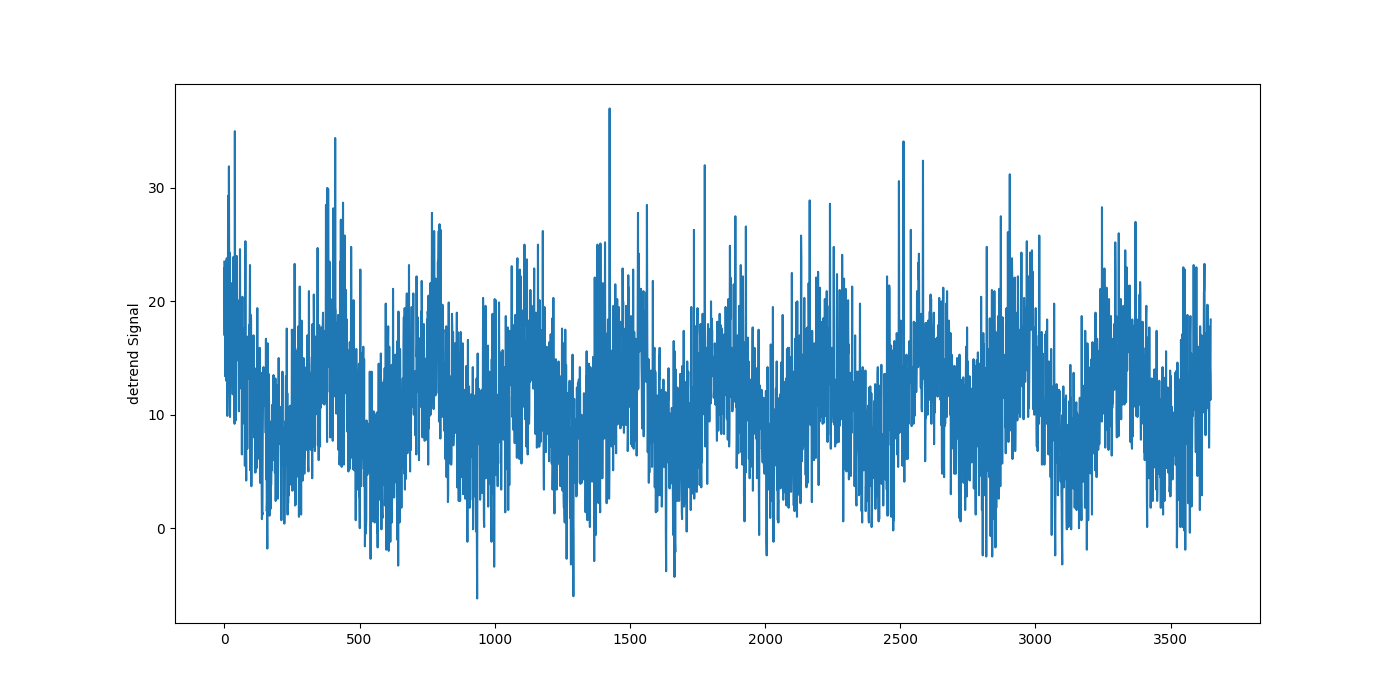
\includegraphics[width=\textwidth]{figures/Ass1/Ass1_D1_one_diff.png}
    \end{minipage}
    \caption{Detrending of the first dataset by the first-order differencing.}
    \label{fig:Ass1_D1_one_diff}
\end{figure}

\begin{figure}[H]
    \centering
    \begin{minipage}[b]{1\textwidth}
        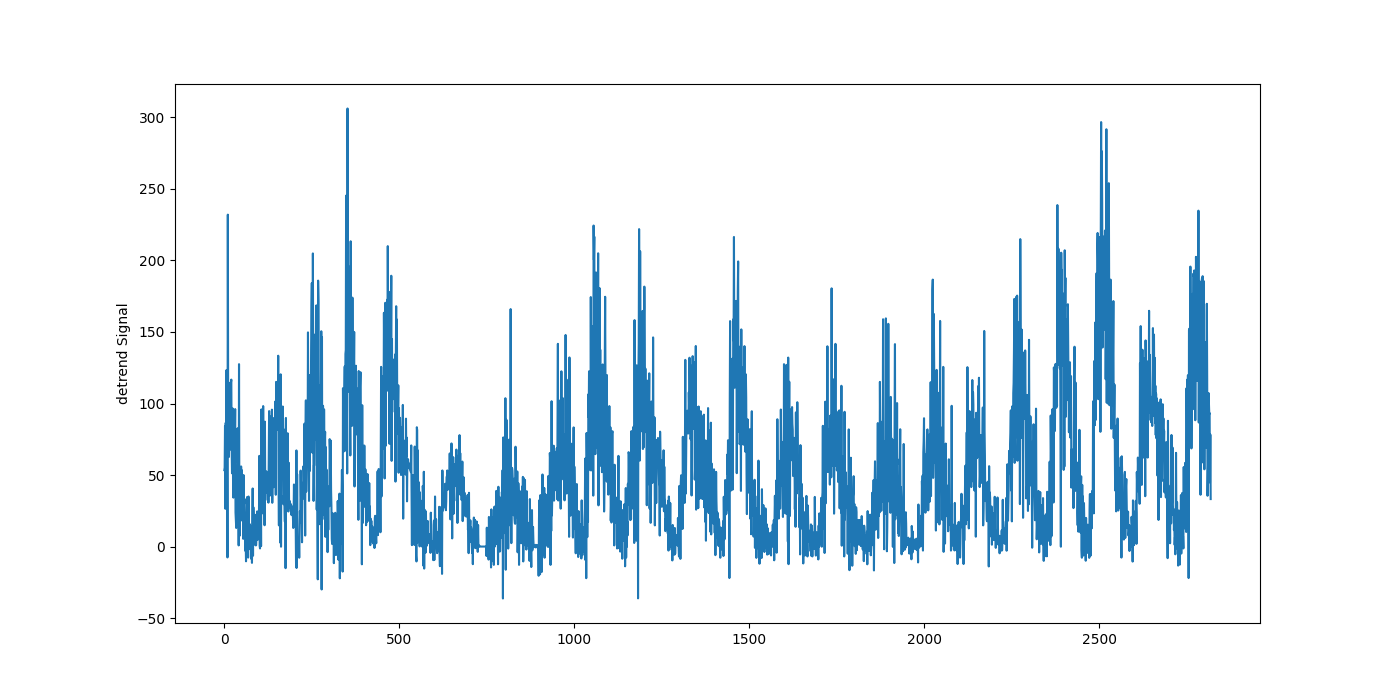
\includegraphics[width=\textwidth]{figures/Ass1/Ass1_D2_one_diff.png}
    \end{minipage}
    \caption{Detrending of the second dataset by the first-order differencing.}
    \label{fig:Ass1_D2_one_diff}
\end{figure}

\begin{figure}[H]
    \centering
    \begin{minipage}[b]{1\textwidth}
        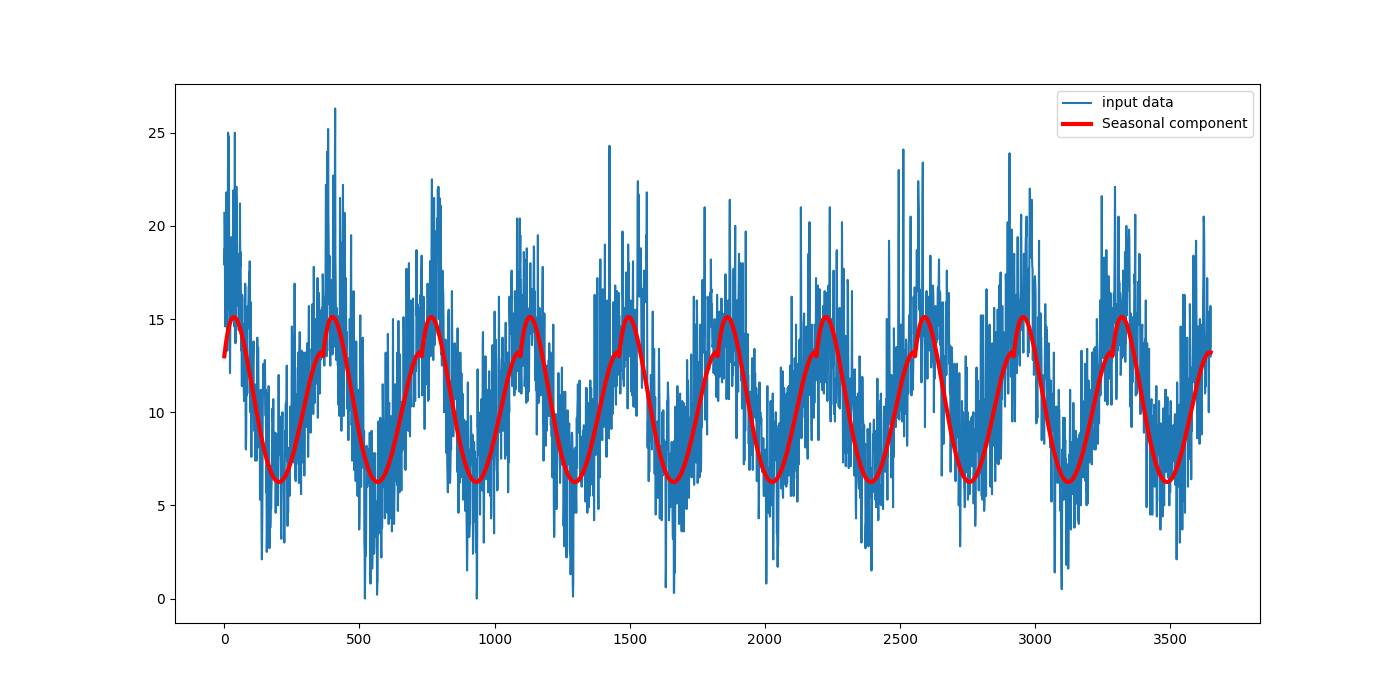
\includegraphics[width=\textwidth]{figures/Ass1/Ass1_D1_fiting_polynomial.png}
    \end{minipage}
    \caption{Seasonal component of the first dataset by fitting a polynomial (Degree of the polynomial is 4).}
    \label{fig:Ass1_D1_fiting_polynomial}
\end{figure}

\begin{figure}[H]
    \centering
    \begin{minipage}[b]{1\textwidth}
        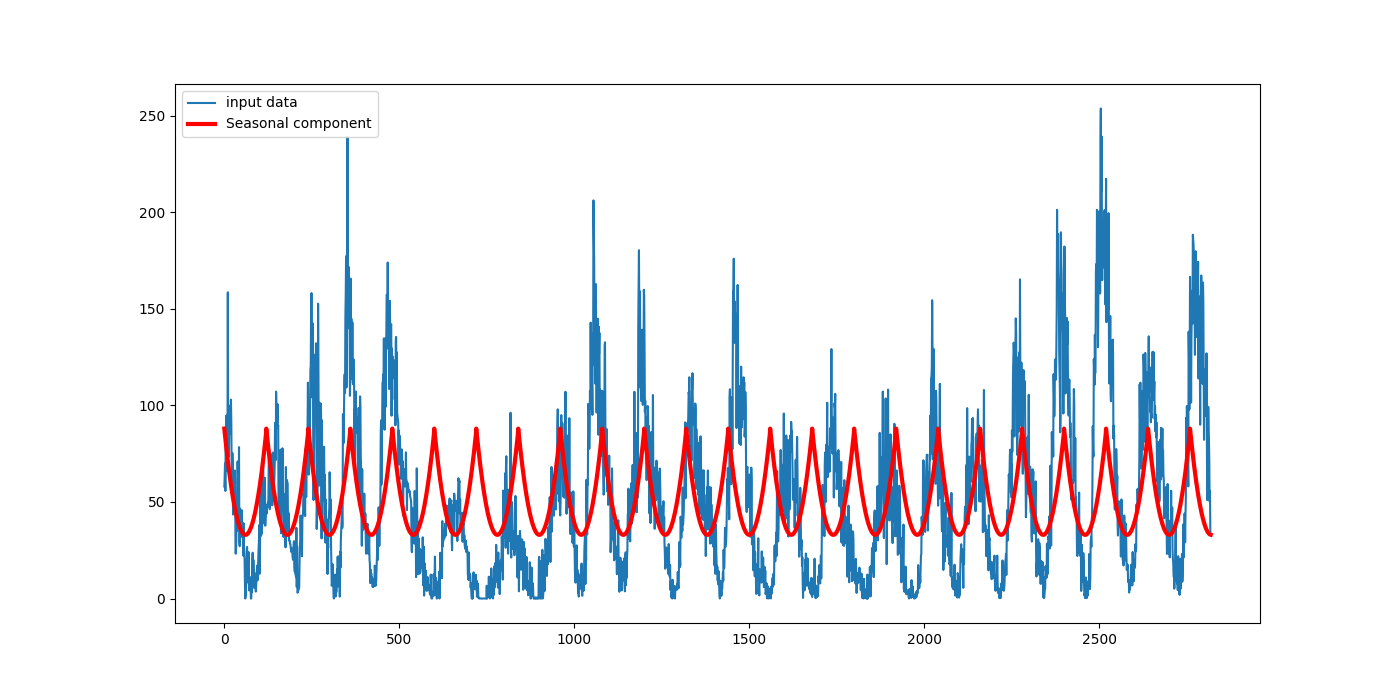
\includegraphics[width=\textwidth]{figures/Ass1/Ass1_D2_fiting_polynomial.png}
    \end{minipage}
    \caption{Seasonal component of the second dataset by fitting a polynomial (Degree of the polynomial is 2).}
    \label{fig:Ass1_D2_fiting_polynomial}
\end{figure}

\begin{figure}[H]
    \centering
    \begin{minipage}[b]{1\textwidth}
        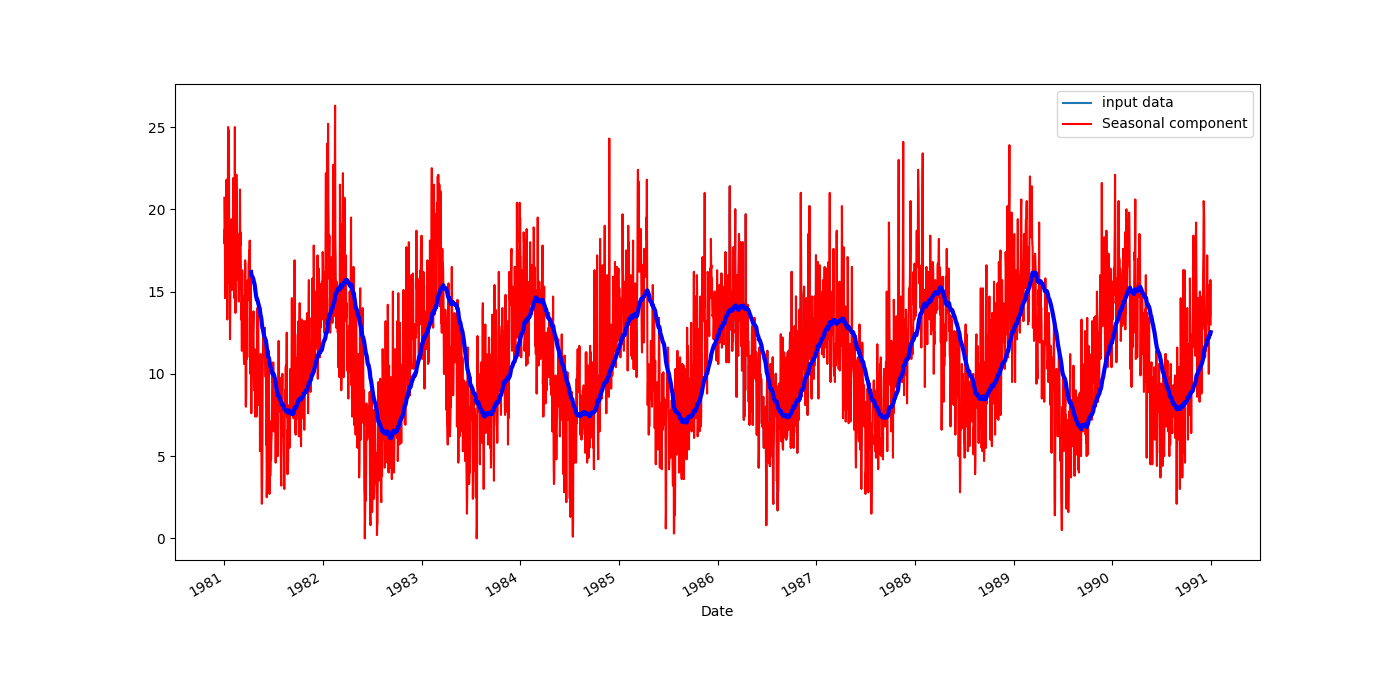
\includegraphics[width=\textwidth]{figures/Ass1/Ass1_D1_Moving_Avrage.png}
    \end{minipage}
    \caption{Seasonal component of the first dataset by Moving Average. The size of the window was set to 100.}
    \label{fig:Ass1_D1_Moving_Avrage}
\end{figure}

\begin{figure}[H]
    \centering
    \begin{minipage}[b]{1\textwidth}
        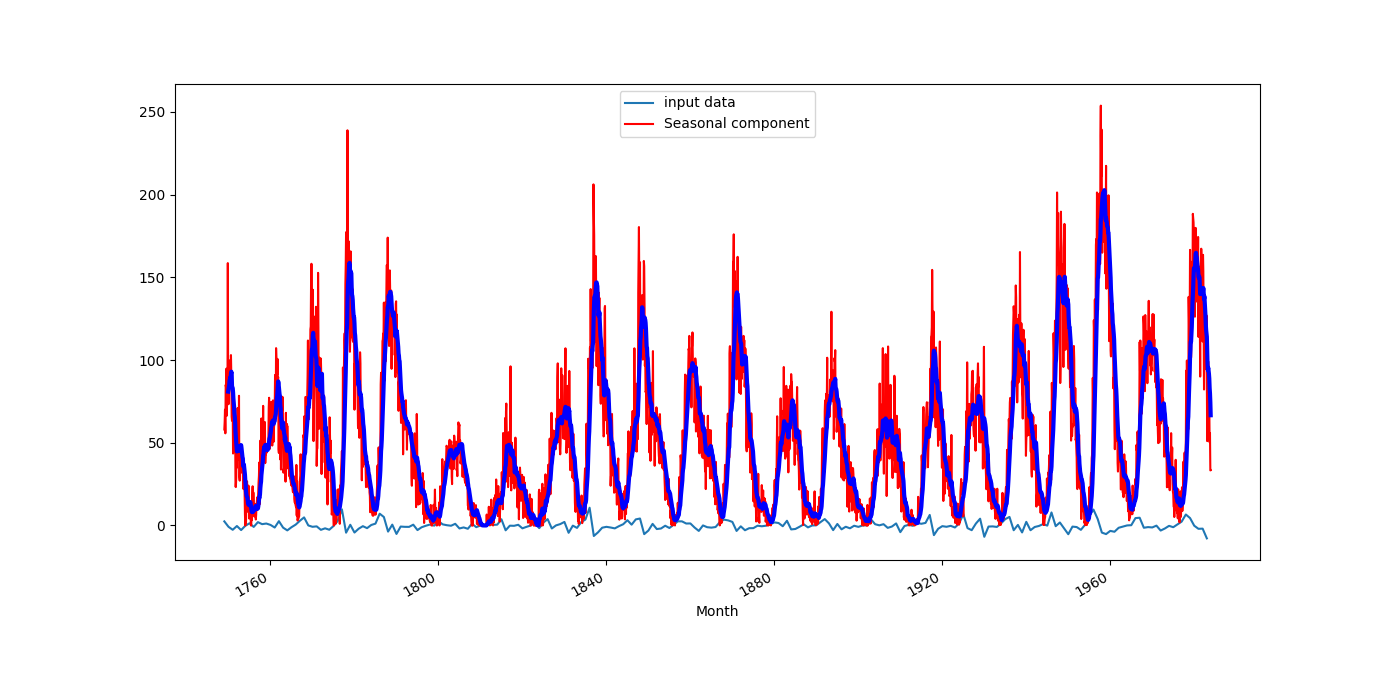
\includegraphics[width=\textwidth]{figures/Ass1/Ass1_D2_Moving_Avrage.png}
    \end{minipage}
    \caption{Seasonal component of the second dataset by Moving Average. The size of the window was set to 12.  }
    \label{fig:Ass1_D2_Moving_Avrage}
\end{figure}




%%%%%%%%%%%%%%%%%%%%%%%%%%%%%%%%%%%%%%%%%%%%%%%%%%%%%%%%%%%%%%%%%
%%%%%%%%%%%%%%%%%%%%%%%% Question 2 %%%%%%%%%%%%%%%%%%%%%%%%%%%%%
%%%%%%%%%%%%%%%%%%%%%%%%%%%%%%%%%%%%%%%%%%%%%%%%%%%%%%%%%%%%%%%%%
\newpage
\item \textbf{For each dataset, examine the stationarity of the residuals using the ACF and PACF functions, Lag Plots, and/or other approaches. Show your results and provide commentary about your observations.}

\textit{\gls{ADF} shows that the time series is non-stationary or stationary. If the p-value is less than the significance level of 0.05 and the \gls{ADF} statistic is lower than one of the critical values, then the time series is stationary. For example, tables \ref{tab:Ass1_D1_ADF} and \ref{tab:Ass1_D2_ADF} shows the result of \gls{ADF} on a residual component of STL method in the two datasets.}

\begin{table}[H]
\centering
\caption{The result of the \gls{ADF} on the first dataset.}
\label{tab:Ass1_D1_ADF}
\begin{tabular}{lr}
\toprule
{} &            0 \\
\midrule
ADF Statistic               &   -24.697687 \\
p-value                     &     0.000000 \\
\#Lags Used                  &     3.000000 \\
Number of Observations Used &  3646.000000 \\
Critical Value (1\%)         &    -3.432145 \\
Critical Value (5\%)         &    -2.862333 \\
Critical Value (10\%)        &    -2.567192 \\
\bottomrule
\end{tabular}

\end{table}

\begin{table}[H]
\centering
\caption{The result of the \gls{ADF} on the second dataset.}
\label{tab:Ass1_D2_ADF}
\begin{tabular}{lr}
\toprule
{} &             0 \\
\midrule
ADF Statistic               & -1.128610e+01 \\
p-value                     &  1.416821e-20 \\
\#Lags Used                  &  2.700000e+01 \\
Number of Observations Used &  2.792000e+03 \\
Critical Value (1\%)         & -3.432694e+00 \\
Critical Value (5\%)         & -2.862576e+00 \\
Critical Value (10\%)        & -2.567321e+00 \\
\bottomrule
\end{tabular}

\end{table}



\textit{\gls{KPSS} is another test for checking the stationarity of a time series. If the p-value is less than the significance level of 0.05, then the time series is not stationary. Table \ref{tab:Ass1_D1_KPSS} and \ref{tab:Ass1_D2_KPSS} show the result of this test on STL residual.}

\begin{table}[H]
\centering
\caption{The result of the \gls{KPSS} on the first dataset.}
\label{tab:Ass1_D1_KPSS}
\begin{tabular}{lr}
\toprule
{} &          0 \\
\midrule
KPSS Statistic        &   0.318117 \\
p-value               &   0.100000 \\
Lags Used             &  22.000000 \\
Critical Value (10\%)  &   0.347000 \\
Critical Value (5\%)   &   0.463000 \\
Critical Value (2.5\%) &   0.574000 \\
Critical Value (1\%)   &   0.739000 \\
\bottomrule
\end{tabular}

\end{table}

\begin{table}[H]
\centering
\caption{The result of the \gls{KPSS} on the second dataset.}
\label{tab:Ass1_D2_KPSS}
\begin{tabular}{lr}
\toprule
{} &          0 \\
\midrule
KPSS Statistic        &   0.017052 \\
p-value               &   0.100000 \\
Lags Used             &  68.000000 \\
Critical Value (10\%)  &   0.347000 \\
Critical Value (5\%)   &   0.463000 \\
Critical Value (2.5\%) &   0.574000 \\
Critical Value (1\%)   &   0.739000 \\
\bottomrule
\end{tabular}

\end{table}

\textit{We can conclude that the series is stationary or not based on both \gls{KPSS} and \gls{ADF} \cite{StationarityStatsmodels}. Table \ref{tab:1} shows the possible outcomes of applying these two tests.}

\begin{table}[H]
\centering
\caption{The combination of the result of the \gls{KPSS} and \gls{ADF}.}
\label{tab:1}
% Please add the following required packages to your document preamble:
% \usepackage[table,xcdraw]{xcolor}
% If you use beamer only pass "xcolor=table" option, i.e. \documentclass[xcolor=table]{beamer}
\centering
\begin{tabular}{|l|l|l|}
\hline
KPSS test      & KDF test       & The combination result                      \\ \hline
non-stationary & non-stationary & The series is non-stationary.               \\ \hline
stationary     & non-stationary & Use detrending to make series stationary.   \\ \hline
non-stationary & stationary     & Use differencing to make series stationary. \\ \hline
stationary     & stationary     & The series is stationary.                   \\ \hline
\end{tabular}

\end{table}



\textit{\gls{ACF}  and \gls{PACF} plots allow you to determine the time series at zero hoe much correlation has with other lags. Figure \ref{fig:Ass1_D1_PACF_ACF} and \ref{fig:Ass1_D2_PACF_ACF} indicate these two plot for our datasets.}



\begin{figure}[H]
    \centering
    \begin{minipage}[b]{1\textwidth}
        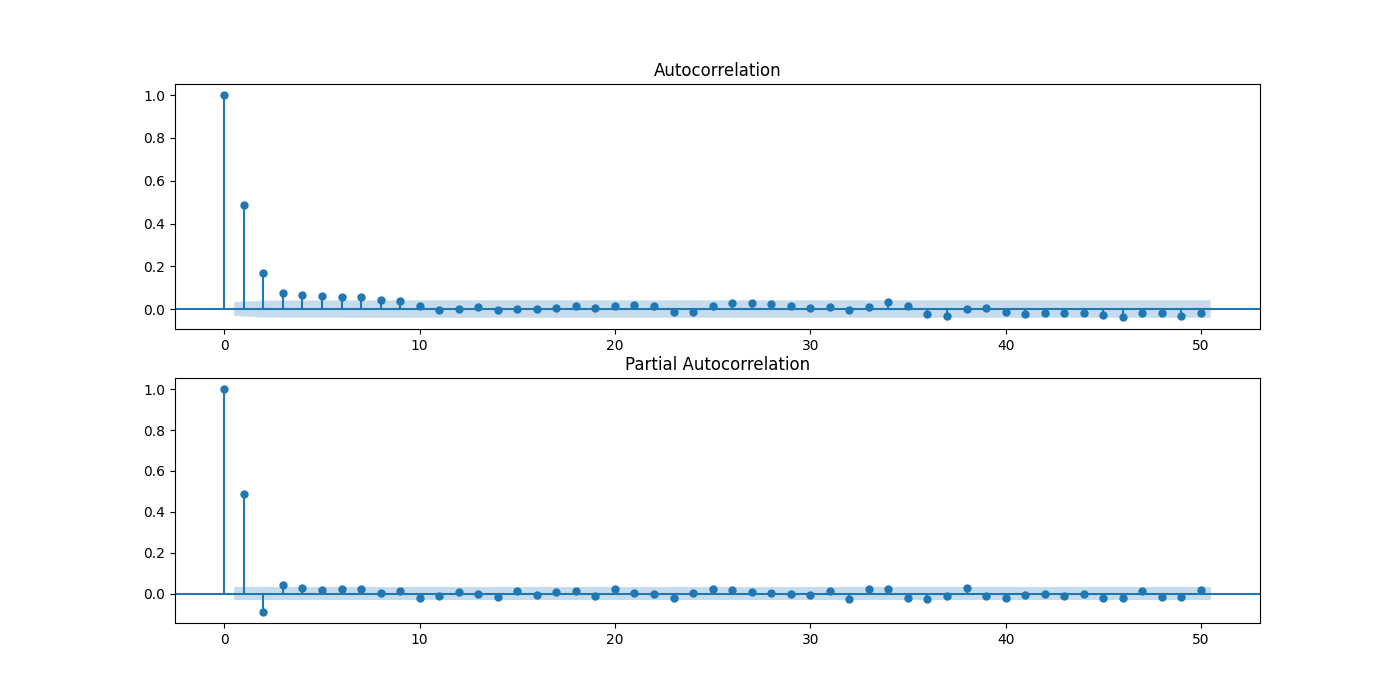
\includegraphics[width=\textwidth]{figures/Ass1/Ass1_D1_PACF_ACF.png}
    \end{minipage}
    \caption{A plot of the \gls{ACF} and \gls{PACF} of the first dataset.}
    \label{fig:Ass1_D1_PACF_ACF}
\end{figure}

\begin{figure}[H]
    \centering
    \begin{minipage}[b]{1\textwidth}
        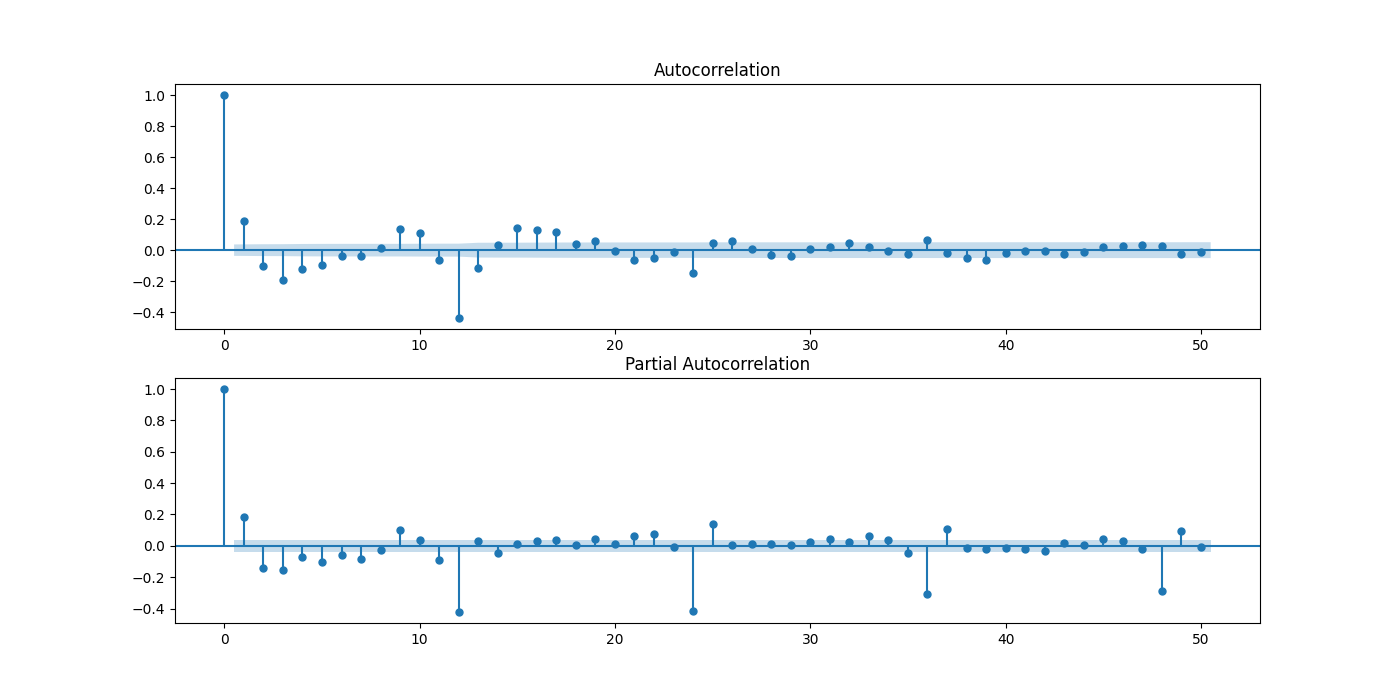
\includegraphics[width=\textwidth]{figures/Ass1/Ass1_D2_PACF_ACF.png}
    \end{minipage}
    \caption{A plot of the \gls{ACF} and \gls{PACF} of the second dataset.}
    \label{fig:Ass1_D2_PACF_ACF}
\end{figure}


\textit{These two plots are used to find the q and p for the ARIMA model. For example, if \gls{ACF} decays towards zero, and \gls{PACF} have only q significant value then our time series is a AR(q) process.}

\begin{table}[H]
\centering
\caption{The combination of the result of the \gls{KPSS} and \gls{ADF}.}
\label{tab:1}
% Please add the following required packages to your document preamble:
% \usepackage[table,xcdraw]{xcolor}
% If you use beamer only pass "xcolor=table" option, i.e. \documentclass[xcolor=table]{beamer}
\centering
\begin{tabular}{|l|l|l|}
\hline
KPSS test      & KDF test       & The combination result                      \\ \hline
non-stationary & non-stationary & The series is non-stationary.               \\ \hline
stationary     & non-stationary & Use detrending to make series stationary.   \\ \hline
non-stationary & stationary     & Use differencing to make series stationary. \\ \hline
stationary     & stationary     & The series is stationary.                   \\ \hline
\end{tabular}

\end{table}

\textit{The below figures (figure \ref{fig:Ass1_D1_Lag_Plots} and \ref{fig:Ass1_D2_Lag_Plots} ) show the lag plot of the two datasets. In each figure, there are four lag plots. As these plots illustrate, both datasets are linear, therefore our time series are a AR process.  }


\begin{figure}[H]
    \centering
    \begin{minipage}[b]{1\textwidth}
        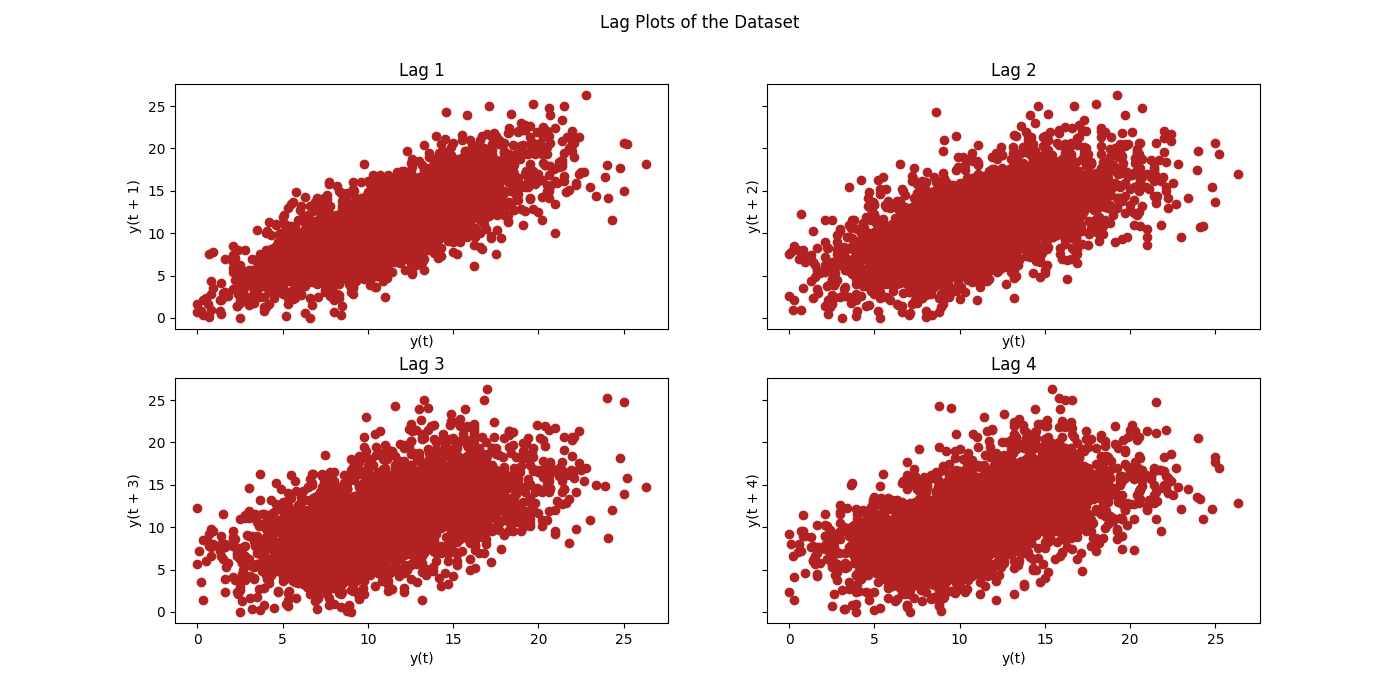
\includegraphics[width=\textwidth]{figures/Ass1/Ass1_D1_Lag_Plots.png}
    \end{minipage}
    \caption{A different lag plot of the first dataset.}
    \label{fig:Ass1_D1_Lag_Plots}
\end{figure}

\begin{figure}[H]
    \centering
    \begin{minipage}[b]{1\textwidth}
        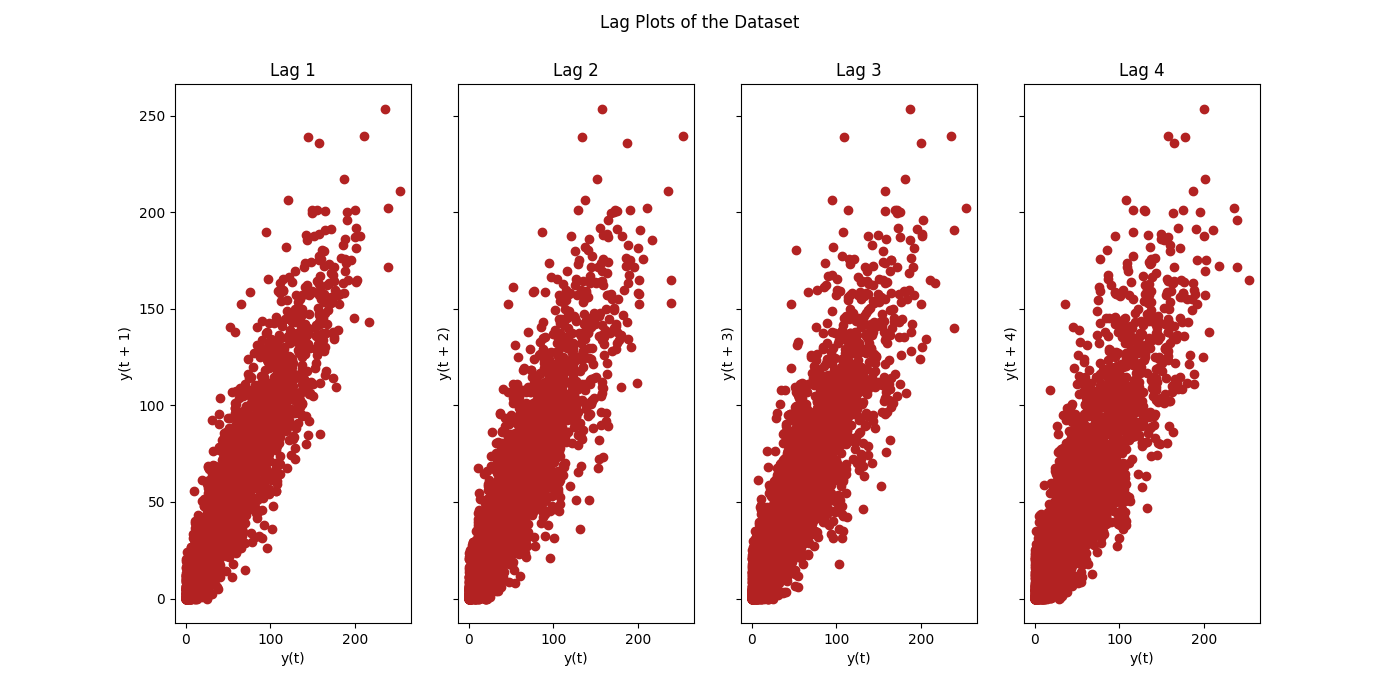
\includegraphics[width=\textwidth]{figures/Ass1/Ass1_D2_Lag_Plots.png}
    \end{minipage}
    \caption{A different lag plot of the second dataset.}
    \label{fig:Ass1_D2_Lag_Plots}
\end{figure}




\begin{figure}[H]
    \centering
    \begin{minipage}[b]{1\textwidth}
        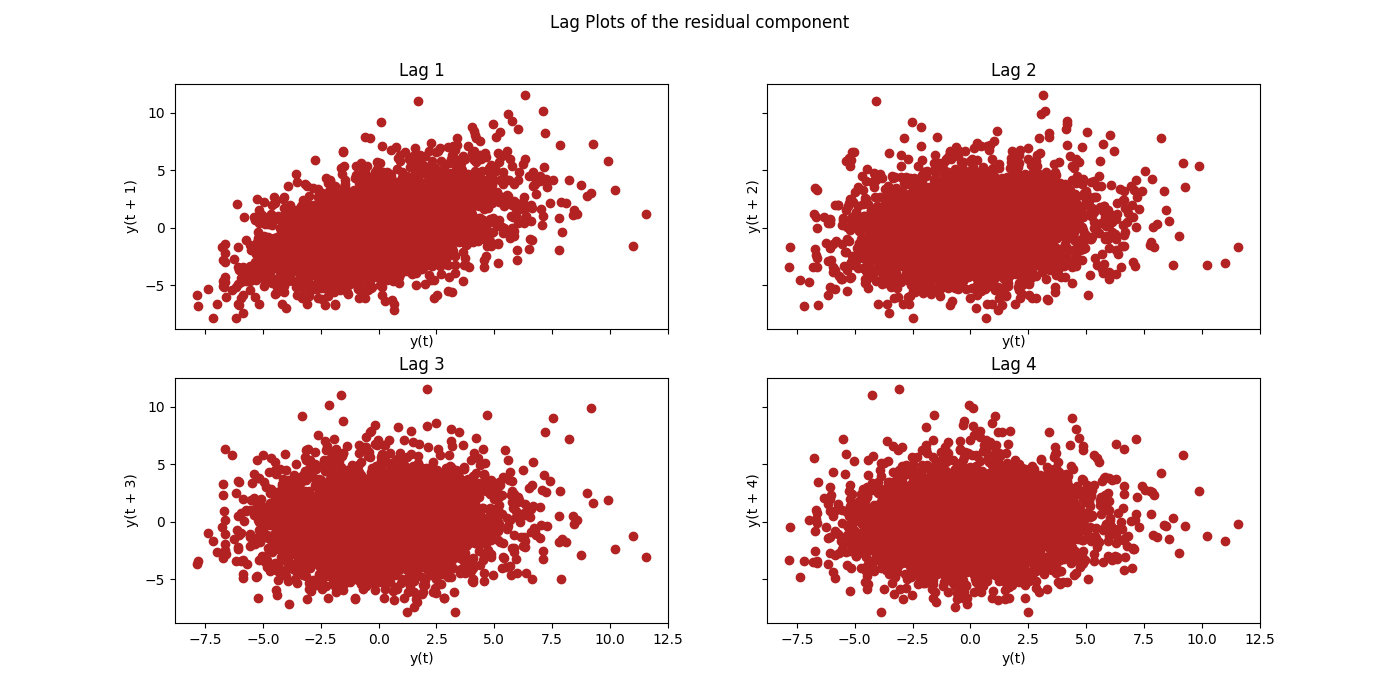
\includegraphics[width=\textwidth]{figures/Ass1/Ass1_D1_Lag_Plots_residual.png}
    \end{minipage}
    \caption{A different lag plot of residual component of the first dataset.}
    \label{fig:Ass1_D1_Lag_Plots_residual}
\end{figure}

\begin{figure}[H]
    \centering
    \begin{minipage}[b]{1\textwidth}
        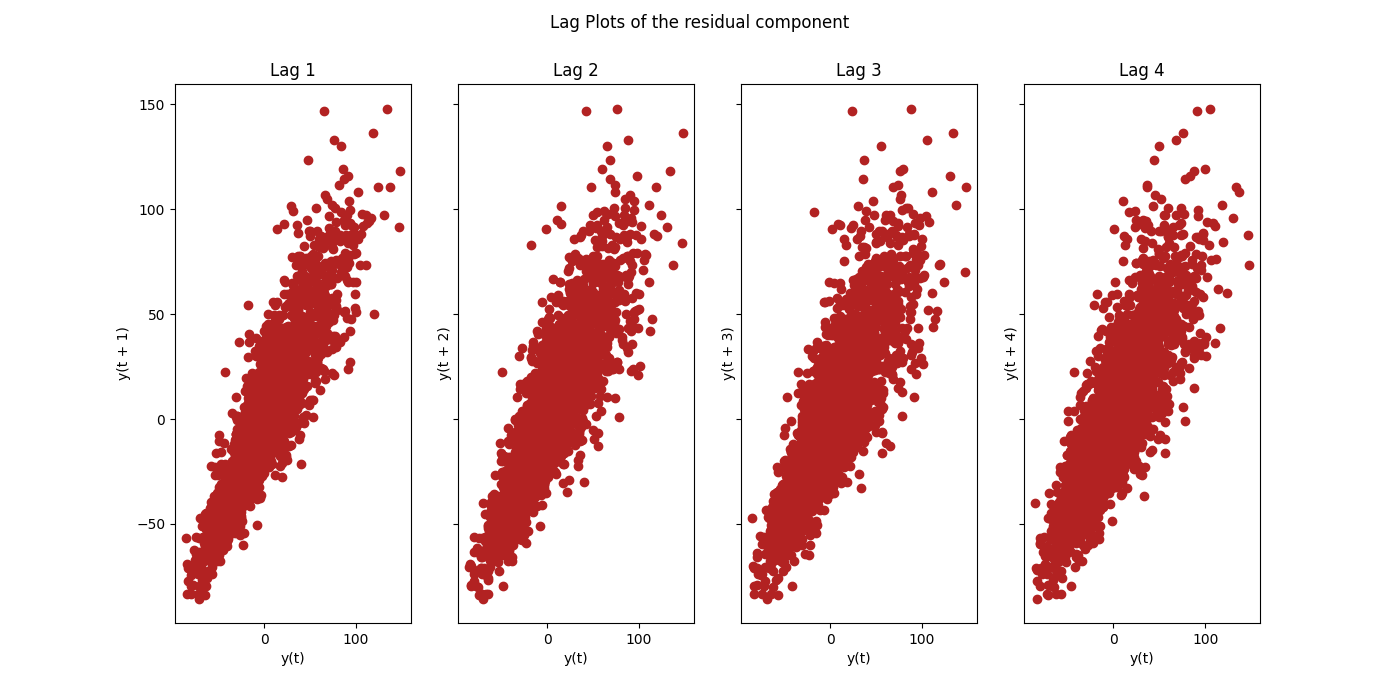
\includegraphics[width=\textwidth]{figures/Ass1/Ass1_D2_Lag_Plots_residual.png}
    \end{minipage}
    \caption{A different lag plot of residual component of the second dataset.}
    \label{fig:Ass1_D2_Lag_Plots_residual}
\end{figure}


%%%%%%%%%%%%%%%%%%%%%%%%%%%%%%%%%%%%%%%%%%%%%%%%%%%%%%%%%%%%%%%%%
%%%%%%%%%%%%%%%%%%%%%%%% Question 3 %%%%%%%%%%%%%%%%%%%%%%%%%%%%%
%%%%%%%%%%%%%%%%%%%%%%%%%%%%%%%%%%%%%%%%%%%%%%%%%%%%%%%%%%%%%%%%%
\newpage
\item \textbf{Try modeling the residuals as an AR process. Use the tools at your disposal to decide on an appropriate order and analyse the results. What is the impact of selecting different orders on the remaining residuals?}

\textit{For this question, we need to select the order of the \gls{AR} term (p). Therefore, \gls{PACF} and \gls{ACF} were plotted at first (see figure \ref{fig:Ass1_D1_PACF_ACF_X}).}  

\begin{figure}[H]
    \centering
    \begin{minipage}[b]{1\textwidth}
        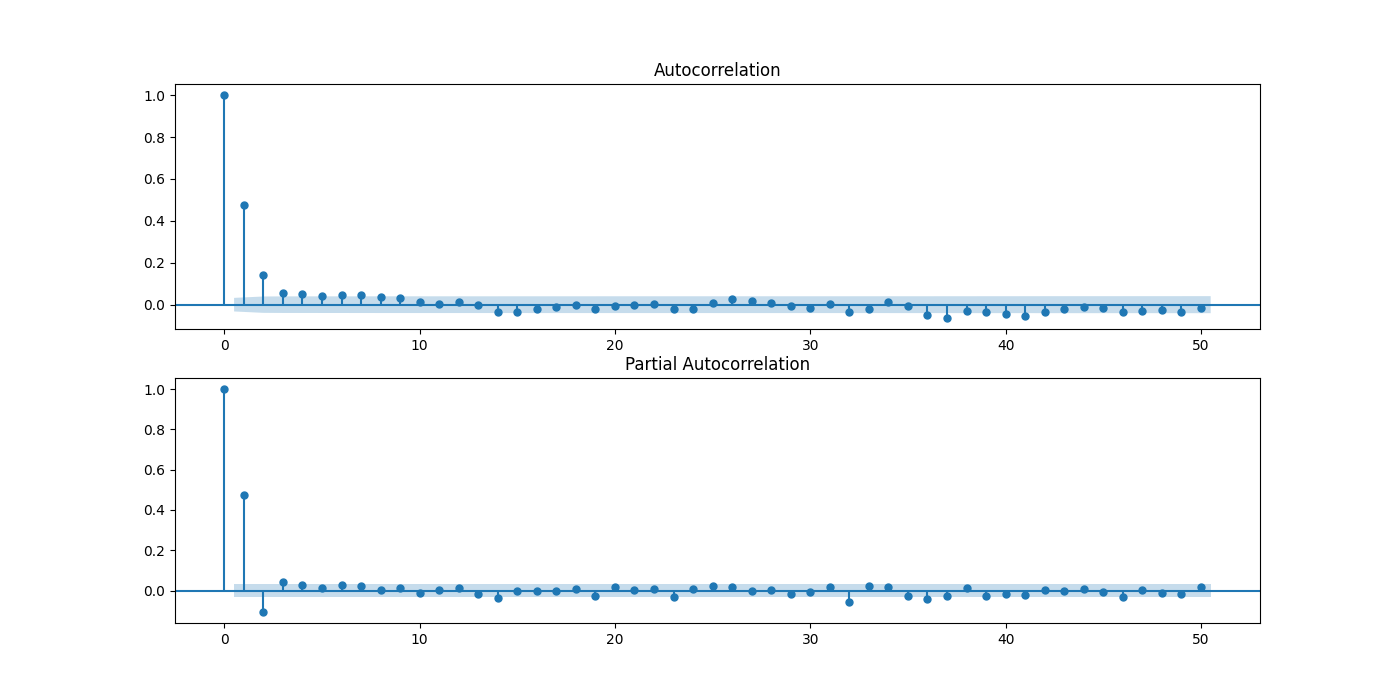
\includegraphics[width=\textwidth]{figures/Ass1/Ass1_D1_PACF_ACF_X.png}
    \end{minipage}
    \caption{A plot of the \gls{PACF} and \gls{ACF} of the residual part of the first dataset (residual of the STL method).}
    \label{fig:Ass1_D1_PACF_ACF_X}
\end{figure}

\textit{Sinse \gls{ACF} decaying (as figure \ref{fig:Ass1_D1_PACF_ACF_X} indicates), it can be concluded that the process is Auto Regressive. Also, based on PACF, the parameter of the \gls{AR} model should be start with an Auto Regressive model with lags 1 and 2 due to these two lags have a significant value.}



based on PACF we should start with an AR model with lags lags 1 ,2 ,10 ,13

so these are my starting points
must be stationary
these two plot do not tell us much


The PACF shows a single spike at the first lag and the ACF shows a tapering pattern. An AR(1) model is indicated.

2.How to find the order of the AR term (p)
\# PACF plot of 1st differenced series


You see how ACF is declining in amplitude exponentially, while PACF cuts off after lag 1. This may suggest that you\'re dealing with AR(1) process.

Note that the ACF shows exponential decay. This is indicative of a stationary series.

Note that the ACF shows an oscillation, indicative of a seasonal series. Note the peaks occur at lags of 12 months, 

The Akaike Information Critera (AIC) is a widely used measure of a statistical model. It basically quantifies 1) the goodness of fit, and 2) the simplicity/parsimony, of the model into a single statistic. When comparing two models, the one with the lower AIC is generally “better”.
%%%%%%%%%%%%%%%%%%%%%%%%%%%%%%%%%%%%%%%%%%%%%%%%%%%%%%%%%%%%%%%%%
%%%%%%%%%%%%%%%%%%%%%%%% Question 4 %%%%%%%%%%%%%%%%%%%%%%%%%%%%%
%%%%%%%%%%%%%%%%%%%%%%%%%%%%%%%%%%%%%%%%%%%%%%%%%%%%%%%%%%%%%%%%%
\newpage
\item \textbf{Summarize your findings and observations briefly in a final discussion. Submit both the developed code and your document to the Assignment 1 folder on D2L.}

\textit{All files were uploaded on my GitHub repository \cite{}. The below table, shows the important paths of the project. Beside the codes are available in Appendix }

\begin{table}[H]
\centering
\begin{tabular}{|l|l|}
\hline
\multicolumn{2}{|l|}{The Important Paths:        } \\ \hline
\ \ \ \    ./EE6563/Dataset/Ass1             & Assignment datasets\\ \hline
\ \ \ \    ./EE6563/code/Ass1/sun.py         & Assignment code\\ \hline
\ \ \ \    ./EE6563/code/Ass1/Temp.py        & Assignment code\\ \hline
\ \ \ \    ./EE6563/manuscript/src/figures   & Assignment figures\\ \hline
\ \ \ \    ./EE6563/manuscript/src/tables    & Assignment table\\ \hline
\ \ \ \    ./EE6563/manuscript/src/Ass1.tex  & Assignment document\\ \hline
\end{tabular}
\end{table}












\end{enumerate}



\newpage
\section*{REFERENCES}
\label{sec:sec6}
\printbibliography[heading=none]

%\bibliography{references}


\newpage
\section*{Appendix (codes)}
\subsection*{The script of sun.py}

\begin{lstlisting}
"""https://www.machinelearningplus.com/time-series/time-series-analysis-python/"""
import warnings

warnings.filterwarnings("ignore")

import math
import os

import matplotlib.pyplot as plt
import numpy as np
import pandas as pd
import statsmodels.api as sm

from pandas.plotting import lag_plot
from sklearn.linear_model import LinearRegression
from sklearn.metrics import mean_squared_error
from statsmodels.graphics.tsaplots import plot_acf, plot_pacf
from statsmodels.tsa import seasonal, stattools
from statsmodels.tsa.ar_model import AutoReg
from statsmodels.tsa.arima_model import ARIMA


plt.rcParams["figure.figsize"] = (14, 7)
a = "Ass1_D2_"

print("[INFO] Setting directories")
project_dir = os.getcwd()
fig_dir = os.path.join(project_dir, "manuscript", "src", "figures", "Ass1")
tbl_dir = os.path.join(project_dir, "manuscript", "src", "tables", "Ass1")
data_dir = os.path.join(project_dir, "Dataset", "Ass1")
dataset_file = os.path.join(data_dir, "monthly-sunspots.csv")
# dataset_file = os.path.join(data_dir, "temperatures.csv")


print("[INFO] Reading the first dataset")
series = pd.read_csv(
    dataset_file,
    header=0,
    index_col=0,
).dropna()

series.index = pd.to_datetime(series.index)

plt.close("all")
############################################################################
#########      Saving and showing the plot of the raw signal      ##########
############################################################################

print("[INFO] Saving and showing the plot of the first dataset")
plt.figure(0)
fig = series.plot()
plt.savefig(os.path.join(fig_dir, a + "raw_signal.png"))


plt.figure()
plt.plot(series["1749":"1800"])
plt.savefig(os.path.join(fig_dir, a + "raw_signal_1990.png"))


series_diff = series.copy(deep=True)
series_diff["Sunspots"] = series.diff().dropna()
series_diff.dropna(inplace=True)
plt.figure()
fig = plt.plot(series_diff)
plt.savefig(os.path.join(fig_dir, a + "1_diff_raw_signal.png"))


series_2diff = series.copy(deep=True)
series_2diff["Sunspots"] = series.diff().diff().dropna()
series_2diff.dropna(inplace=True)
fig = plt.plot(series_2diff)
plt.savefig(os.path.join(fig_dir, a + "2_diff_raw_signal.png"))


print("[INFO] Saving and printing the head of the first dataset")
with open(os.path.join(tbl_dir, a + "raw_signal.tex"), "w") as tf:
    tf.write(series.head(5).to_latex())


print(series.describe())
with open(os.path.join(tbl_dir, a + "raw_signal_summary_statistics.tex"), "w") as tf:
    tf.write(series.describe().to_latex())

############################################################################
#########        Decompositions: Moving Avarage function          ##########
############################################################################
print("[INFO] Saving and showing the plot of Moving Avarage function")

# r.agg, r.apply, r.count, r.exclusions, r.max, r.median, r.name, r.quantile, r.kurt, r.cov, r.corr, r.aggregate, r.std, r.skew, r.sum, r.var
r = series.rolling(window=12)

plt.figure()
axes = plt.axes()
series.plot(color="red", ax=axes)
r.mean().plot(style="b", linewidth=3, ax=axes)

plt.legend(["input data", "Seasonal component"])
plt.savefig(os.path.join(fig_dir, a + "Moving_Avrage.png"))


############################################################################
#########        Decompositions: seasonal_decompose method        ##########
############################################################################

print("[INFO] Plot the decomposition by seasonal_decompose method...")
decomposition_sd = seasonal.seasonal_decompose(
    series, model="additive", extrapolate_trend="freq"  # , period=120
)

fig = decomposition_sd.plot()
plt.savefig(os.path.join(fig_dir, a + "seasonal_decompose.png"))


############################################################################
#########          Seasonal Modeling (fitting polynomial)         ##########
############################################################################
resample = series.resample("AS").mean()
plt.figure()
plt.plot(resample)
plt.savefig(os.path.join(fig_dir, a + "resample.png"))


print("[INFO] Plot the decomposition by fitting polynomial method...")
X = [i % 120 for i in range(0, len(series))]
y = series.values

degree = 2
coef = np.polyfit(X, y, degree)
print("[INFO] polynomial Coefficients are :\n%s\n" % coef)


curve = list()
for i in range(len(X)):
    value = 88
    for d in range(degree):
        value += X[i] ** (degree - d) * coef[d]
    curve.append(value)

plt.figure()
plt.plot(y)
plt.plot(curve, color="red", linewidth=3)
plt.legend(["input data", "Seasonal component"])
plt.savefig(os.path.join(fig_dir, a + "fiting_polynomial.png"))


############################################################################
#########          Decompositions: Differencing method            ##########
############################################################################
print("[INFO] Plot the detrending signal by Differencing method...")
diff = list()
period = 1
for i in range(period, len(X)):
    value = series.values[i] - series.values[i - period]
    diff.append(value)

plt.figure()
plt.plot(series.values[:-1] - diff)
plt.ylabel("detrend Signal")
plt.savefig(os.path.join(fig_dir, a + "one_diff.png"))


############################################################################
#########               Decompositions: STL method                ##########
############################################################################

print("[INFO] Plot the decomposition by STL method...")
decomposition_STL = seasonal.STL(series, period=130).fit()
fig = decomposition_STL.plot()
plt.savefig(os.path.join(fig_dir, a + "STL.png"))


############################################################################
#########         Decompositions: LinearRegression method         ##########
############################################################################

print("[INFO] Plot the decomposition by LinearRegression method...")
X = [i for i in range(0, len(series))]
X = np.reshape(X, (len(X), 1))
y = series.values
model = LinearRegression()
model.fit(X, y)
trend = model.predict(X)

# plot the raw signal
plt.subplot(411)
plt.plot(y)
plt.ylabel("the raw signal")

# plot trend
plt.subplot(412)
plt.plot(trend)
plt.ylabel("trend")
# detrending
detrended = [y[i] - trend[i] for i in range(0, len(series))]
# plot Detrended
plt.subplot(413)
plt.plot(detrended)
plt.ylabel("seasonal")

############################################################################
#########          Decompositions: Differencing method            ##########
############################################################################
"""https://machinelearningmastery.com/time-series-seasonality-with-python/"""
print("[INFO] Plot the seasonal signal by Differencing method...")

diff = list()
period = 120
for i in range(period, len(X)):
    value = detrended[i] - detrended[i - period]
    diff.append(value)

# plot Residual
plt.subplot(414)
plt.plot(diff)
plt.ylabel("residual")
plt.savefig(os.path.join(fig_dir, a + "LinearRegression_diff.png"))


############################################################################
#########               stationary test: ADF method               ##########
############################################################################

"""residual = {decomposition_sd.resid, decomposition_STL.resid, diff}"""
residual = decomposition_STL.resid

print("[INFO] ACF plot for residual component...")
plt.figure()
plot_acf(residual, lags=100)
plt.savefig(os.path.join(fig_dir, a + "ACF.png"))

print("[INFO] Results of Dickey-Fuller Test:")
result = stattools.adfuller(residual, autolag="AIC")
dfoutput = pd.Series(
    result[0:4],
    index=["ADF Statistic", "p-value", "#Lags Used", "Number of Observations Used"],
)
for key, value in result[4].items():
    dfoutput["Critical Value (%s)" % key] = value
print(dfoutput)

print("[INFO] saving Results of Dickey-Fuller Test on file...")
with open(os.path.join(tbl_dir, a + "ADF.tex"), "w") as tf:
    tf.write(dfoutput.to_latex(index=True))


print("[INFO] ACF plot for the first order diff...")
plt.figure()
plot_acf(series_diff, lags=100)
plt.savefig(os.path.join(fig_dir, a + "ACF_1_diff.png"))

print("[INFO] Results of Dickey-Fuller Test:")
result = stattools.adfuller(series_diff, autolag="AIC")
dfoutput = pd.Series(
    result[0:4],
    index=["ADF Statistic", "p-value", "#Lags Used", "Number of Observations Used"],
)
for key, value in result[4].items():
    dfoutput["Critical Value (%s)" % key] = value
print(dfoutput)

print("[INFO] saving Results of Dickey-Fuller Test on file...")
with open(os.path.join(tbl_dir, a + "ADF_1_diff.tex"), "w") as tf:
    tf.write(dfoutput.to_latex(index=True))


print("[INFO] ACF plot for the second order diff...")
plt.figure()
plot_acf(series_2diff, lags=100)
plt.savefig(os.path.join(fig_dir, a + "ACF_2_diff.png"))

print("[INFO] Results of Dickey-Fuller Test:")
result = stattools.adfuller(series_2diff, autolag="AIC")
dfoutput = pd.Series(
    result[0:4],
    index=["ADF Statistic", "p-value", "#Lags Used", "Number of Observations Used"],
)
for key, value in result[4].items():
    dfoutput["Critical Value (%s)" % key] = value
print(dfoutput)

print("[INFO] saving Results of Dickey-Fuller Test on file...")
with open(os.path.join(tbl_dir, a + "ADF_2_diff.tex"), "w") as tf:
    tf.write(dfoutput.to_latex(index=True))


############################################################################
#########              stationary test: KPSS method               ##########
############################################################################
"""
## https://www.statsmodels.org/stable/examples/notebooks/generated/stationarity_detrending_adf_kpss.html
"""
print("[INFO] Results of KPSS Test:")
Results = stattools.kpss(residual, regression="c", nlags="auto")
kpss_output = pd.Series(Results[0:3], index=["KPSS Statistic", "p-value", "Lags Used"])
for key, value in Results[3].items():
    kpss_output["Critical Value (%s)" % key] = value
print(kpss_output)

print("[INFO] saving Results of KPSS Test on file...")
with open(os.path.join(tbl_dir, a + "KPSS.tex"), "w") as tf:
    tf.write(kpss_output.to_latex(index=True))


print("[INFO] Results of KPSS Test:")
Results = stattools.kpss(series_diff, regression="c", nlags="auto")
kpss_output = pd.Series(Results[0:3], index=["KPSS Statistic", "p-value", "Lags Used"])
for key, value in Results[3].items():
    kpss_output["Critical Value (%s)" % key] = value
print(kpss_output)

print("[INFO] saving Results of KPSS Test on file...")
with open(os.path.join(tbl_dir, a + "KPSS_1_diff.tex"), "w") as tf:
    tf.write(kpss_output.to_latex(index=True))

print("[INFO] Results of KPSS Test:")
Results = stattools.kpss(series_2diff, regression="c", nlags="auto")
kpss_output = pd.Series(Results[0:3], index=["KPSS Statistic", "p-value", "Lags Used"])
for key, value in Results[3].items():
    kpss_output["Critical Value (%s)" % key] = value
print(kpss_output)

print("[INFO] saving Results of KPSS Test on file...")
with open(os.path.join(tbl_dir, a + "KPSS_2_diff.tex"), "w") as tf:
    tf.write(kpss_output.to_latex(index=True))

############################################################################
#########               stationary test: PACF method              ##########
############################################################################
""" https://towardsdatascience.com/detecting-stationarity-in-time-series-data-d29e0a21e638
"""
print("[INFO] PACF plot for residual component...")
PACF_output = stattools.pacf(residual)
plt.figure()
plt.stem(PACF_output)
plt.savefig(os.path.join(fig_dir, a + "PACF.png"))

plt.figure()
fig, axes = plt.subplots(2, 1)
plot_acf(residual, lags=50, ax=axes[0])
plot_pacf(residual, lags=50, ax=axes[1])
plt.savefig(os.path.join(fig_dir, a + "PACF_ACF.png"))

plt.figure()
fig, axes = plt.subplots(2, 1)
plot_acf(series_diff, lags=50, ax=axes[0])
plot_pacf(series_diff, lags=50, ax=axes[1])
plt.savefig(os.path.join(fig_dir, a + "PACF_ACF_1_diff.png"))

plt.figure()
fig, axes = plt.subplots(2, 1)
plot_acf(series, lags=150, ax=axes[0])
plot_pacf(series, lags=150, ax=axes[1])
plt.savefig(os.path.join(fig_dir, a + "PACF_ACF_series.png"))
############################################################################
#########               stationary test: Lag Plots                ##########
############################################################################

print("[INFO] Lag plot for residual component...")

fig, axes = plt.subplots(2, 2, sharex=True, sharey=True, dpi=100)
for i, ax in enumerate(axes.flatten()[:4]):
    lag_plot(series, lag=i + 1, ax=ax, c="firebrick")
    ax.set_title("Lag " + str(i + 1))

fig.suptitle("Lag Plots of the Dataset")
plt.savefig(os.path.join(fig_dir, a + "Lag_Plots.png"))


fig, axes = plt.subplots(2, 2, sharex=True, sharey=True, dpi=100)
for i, ax in enumerate(axes.flatten()[:4]):
    lag_plot(residual, lag=i + 1, ax=ax, c="firebrick")
    ax.set_title("Lag " + str(i + 1))

fig.suptitle("Lag Plots of the residual component")
plt.savefig(os.path.join(fig_dir, a + "Lag_Plots_residual.png"))

fig, axes = plt.subplots(2, 2, sharex=True, sharey=True, dpi=100)
for i, ax in enumerate(axes.flatten()[:4]):
    lag_plot(series_diff, lag=i + 1, ax=ax, c="firebrick")
    ax.set_title("Lag " + str(i + 1))

fig.suptitle("Lag Plots of the first order diff")
plt.savefig(os.path.join(fig_dir, a + "Lag_Plots_1_diff.png"))

fig, axes = plt.subplots(2, 2, sharex=True, sharey=True, dpi=100)
for i, ax in enumerate(axes.flatten()[:4]):
    lag_plot(series_2diff, lag=i + 1, ax=ax, c="firebrick")
    ax.set_title("Lag " + str(i + 1))

fig.suptitle("Lag Plots of the second order diff")
plt.savefig(os.path.join(fig_dir, a + "Lag_Plots_2_diff.png"))
############################################################################
#########           Predict Approach of Auto Regression           ##########
############################################################################
"""
https://towardsdatascience.com/trend-seasonality-moving-average-auto-regressive-model-my-journey-to-time-series-data-with-edc4c0c8284b
"""


X = decomposition_STL.resid.values

plt.figure()
fig, axes = plt.subplots(2, 1)
plot_acf(X, lags=50, ax=axes[0])
plot_pacf(X, lags=50, ax=axes[1])
plt.savefig(os.path.join(fig_dir, a + "PACF_ACF_X.png"))


print("[INFO] spliting dataset to train and test set...")
n_predict = 14
train, test = X[1 : len(X) - n_predict], X[len(X) - n_predict :]

ar_orders = [1, 2, 3, 4]
fitted_model_dict = {}

AIC_list = list()
BIC_list = list()
RMS_list = list()
cof_list = list()
ord_list = list()
col_list = list()
mae_list = list()
mpe_list = list()
cor_list = list()


for idx, ar_order in enumerate(ar_orders):

    print("[INFO] train autoregression...")
    model = ARIMA(train, order=(ar_order, 0, 0))
    model_fit = model.fit()

    fitted_model_dict[ar_order] = model_fit

    col_list.append("AR({:1.0f})".format(ar_order))

    predictions = model_fit.predict(
        start=len(train), end=len(train) + len(test) - 1, dynamic=False
    )

    RMS_list.append("{:2.3f}".format(np.sqrt(mean_squared_error(test, predictions))))
    mae_list.append("{:2.3f}".format(np.mean(np.abs(predictions - test))))
    mpe_list.append("{:2.3f}".format(np.mean((predictions - test) / test)))
    cor_list.append("{:2.3f}".format(np.corrcoef(predictions, test)[0, 1]))

    plt.figure()
    xpos = np.arange(len(X))
    plt.plot(X[2700:], "r", linewidth=0.5)
    plt.plot(
        xpos[len(X) - n_predict - 2700 : len(X) - 2700], predictions[:], color="blue"
    )
    plt.legend(["train+Test", "Predictions"])
    plt.savefig(os.path.join(fig_dir, a + "_" + str(idx + 1) + "_AR2.png"))

for idx, ar_order in enumerate(ar_orders):
    plt.figure(0)
    plt.subplot(len(ar_orders), 1, idx + 1)
    plt.plot(train[:100])
    plt.plot(fitted_model_dict[ar_order].fittedvalues[:100])
    plt.title("AR({:1.0f}) Fit".format(ar_order), fontsize=16)


plt.tight_layout()
plt.savefig(os.path.join(fig_dir, a + "ARs models.png"))

print("[INFO] AIC and BIC of autoregression models...")
for ar_order in ar_orders:
    AIC_list.append("{:2.3f}".format(fitted_model_dict[ar_order].aic))
    cof_list.append(fitted_model_dict[ar_order].params)
    ord_list.append(ar_order)
    BIC_list.append("{:2.3f}".format(fitted_model_dict[ar_order].bic))


df = pd.DataFrame(
    np.row_stack(
        [ord_list, AIC_list, BIC_list, RMS_list, cor_list, mpe_list, mae_list]
    ),
    index=["lag(s)", "AIC", "BIC", "RMS error", "Correlation", "MPE", "MAE"],
)
df.columns = col_list
print(df)
with open(os.path.join(tbl_dir, a + "AR.tex"), "w") as tf:
    tf.write(df.to_latex(index=True))
\end{lstlisting}
\subsection*{The script of Temp.py}
\begin{lstlisting}
"""https://www.machinelearningplus.com/time-series/time-series-analysis-python/"""
import warnings

warnings.filterwarnings("ignore")

import math
import os

import matplotlib.pyplot as plt
import numpy as np
import pandas as pd
import statsmodels.api as sm
import seaborn as sns

from pandas.plotting import lag_plot
from sklearn.linear_model import LinearRegression
from sklearn.metrics import mean_squared_error
from statsmodels.graphics.tsaplots import plot_acf, plot_pacf
from statsmodels.tsa import seasonal, stattools
from statsmodels.tsa.ar_model import AutoReg
from statsmodels.tsa.arima_model import ARIMA


plt.rcParams["figure.figsize"] = (14, 7)
a = "Ass1_D1_"

print("[INFO] Setting directories")
project_dir = os.getcwd()
fig_dir = os.path.join(project_dir, "manuscript", "src", "figures", "Ass1")
tbl_dir = os.path.join(project_dir, "manuscript", "src", "tables", "Ass1")
data_dir = os.path.join(project_dir, "Dataset", "Ass1")
# dataset_file = os.path.join(data_dir, "monthly-sunspots.csv")
dataset_file = os.path.join(data_dir, "temperatures.csv")


print("[INFO] Reading the first dataset")
series = pd.read_csv(
    dataset_file,
    header=0,
    index_col=0,
).dropna()

series.index = pd.to_datetime(series.index)


############################################################################
#########      Saving and showing the plot of the raw signal      ##########
############################################################################

print("[INFO] Saving and showing the plot of the first dataset")
plt.figure(0)
fig = series.plot()
plt.savefig(os.path.join(fig_dir, a + "raw_signal.png"))

plt.figure()
plt.plot(series["1990":"1991"])
plt.savefig(os.path.join(fig_dir, a + "raw_signal_1990.png"))

plt.figure()
plt.plot(series.loc["1986"])
plt.savefig(os.path.join(fig_dir, a + "raw_signal_1986.png"))


print("[INFO] Saving and printing the head of the first dataset")
with open(os.path.join(tbl_dir, a + "raw_signal.tex"), "w") as tf:
    tf.write(series.head(5).to_latex())


print(series.describe())
with open(os.path.join(tbl_dir, a + "raw_signal_summary_statistics.tex"), "w") as tf:
    tf.write(series.describe().to_latex())

############################################################################
#########         Decompositions: Moving Avrage function          ##########
############################################################################
print("[INFO] Saving and showing the plot of Moving Avrage function")

# r.agg, r.apply, r.count, r.exclusions, r.max, r.median, r.name, r.quantile, r.kurt, r.cov, r.corr, r.aggregate, r.std, r.skew, r.sum, r.var
r = series.rolling(window=100)

plt.figure()
axes = plt.axes()
series.plot(color="red", ax=axes)
r.mean().plot(style="b", linewidth=3, ax=axes)

plt.legend(["input data", "Seasonal component"])
plt.savefig(os.path.join(fig_dir, a + "Moving_Avrage.png"))


############################################################################
#########        Decompositions: seasonal_decompose method        ##########
############################################################################

print("[INFO] Plot the decomposition by seasonal_decompose method...")
decomposition_sd = seasonal.seasonal_decompose(
    series, model="additive", extrapolate_trend="freq", period=365
)

fig = decomposition_sd.plot()
plt.savefig(os.path.join(fig_dir, a + "seasonal_decompose.png"))


############################################################################
#########          Seasonal Modeling (fiting polynomial)          ##########
############################################################################

resample = series.resample("M").mean()
plt.figure()
plt.plot(resample)
plt.savefig(os.path.join(fig_dir, a + "resample.png"))


print("[INFO] Plot the decomposition by fiting polynomial method...")
X = [i % 365 for i in range(0, len(series))]
y = series.values

degree = 5
coef = np.polyfit(X, y, degree)
print("[INFO] polynomial Coefficients are :\n%s\n" % coef)


curve = list()
for i in range(len(X)):
    value = 13
    for d in range(degree):
        value += X[i] ** (degree - d) * coef[d]
    curve.append(value)

plt.figure()
plt.plot(y)
plt.plot(curve, color="red", linewidth=3)
plt.legend(["input data", "Seasonal component"])
plt.savefig(os.path.join(fig_dir, a + "fiting_polynomial.png"))


############################################################################
#########          Decompositions: Differencing method            ##########
############################################################################
print("[INFO] Plot the detrending signal by Differencing method...")
diff = list()
period = 1
for i in range(period, len(X)):
    value = series.values[i] - series.values[i - period]
    diff.append(value)

plt.figure()
plt.plot(series.values[:-1] - diff)
plt.ylabel("detrend Signal")
plt.savefig(os.path.join(fig_dir, a + "one_diff.png"))


############################################################################
#########               Decompositions: STL method                ##########
############################################################################

print("[INFO] Plot the decomposition by STL method...")
decomposition_STL = seasonal.STL(series, period=365).fit()
fig = decomposition_STL.plot()
plt.savefig(os.path.join(fig_dir, a + "STL.png"))


############################################################################
#########         Decompositions: LinearRegression method         ##########
############################################################################

print("[INFO] Plot the decomposition by LinearRegression method...")
X = [i for i in range(0, len(series))]
X = np.reshape(X, (len(X), 1))
y = series.values
model = LinearRegression()
model.fit(X, y)
trend = model.predict(X)

# plot the raw signal
plt.subplot(411)
plt.plot(y)
plt.ylabel("the raw signal")

# plot trend
plt.subplot(412)
plt.plot(trend)
plt.ylabel("trend")
# detrending
detrended = [y[i] - trend[i] for i in range(0, len(series))]
# plot Detrended
plt.subplot(413)
plt.plot(detrended)
plt.ylabel("seasonal")

############################################################################
#########          Decompositions: Differencing method            ##########
############################################################################
"""https://machinelearningmastery.com/time-series-seasonality-with-python/"""
print("[INFO] Plot the seasonal signal by Differencing method...")

diff = list()
period = 365
for i in range(period, len(X)):
    value = detrended[i] - detrended[i - period]
    diff.append(value)

# plot Residual
plt.subplot(414)
plt.plot(diff)
plt.ylabel("residual")
plt.savefig(os.path.join(fig_dir, a + "LinearRegression_diff.png"))


############################################################################
#########               stationary test: ADF method               ##########
############################################################################

"""residual = {decomposition_sd.resid, decomposition_STL.resid, diff}"""
residual = decomposition_sd.resid

print("[INFO] ACF plot for residual component...")
plt.figure()
plot_acf(residual, lags=100)
plt.savefig(os.path.join(fig_dir, a + "ADF.png"))

print("[INFO] Results of Dickey-Fuller Test:")
result = stattools.adfuller(residual, autolag="AIC")
dfoutput = pd.Series(
    result[0:4],
    index=["ADF Statistic", "p-value", "#Lags Used", "Number of Observations Used"],
)
for key, value in result[4].items():
    dfoutput["Critical Value (%s)" % key] = value
print(dfoutput)

print("[INFO] saving Results of Dickey-Fuller Test on file...")
with open(os.path.join(tbl_dir, a + "ADF.tex"), "w") as tf:
    tf.write(dfoutput.to_latex(index=True))

############################################################################
#########              stationary test: KPSS method               ##########
############################################################################

print("[INFO] Results of KPSS Test:")
Results = stattools.kpss(residual, regression="c", nlags="auto")
kpss_output = pd.Series(Results[0:3], index=["KPSS Statistic", "p-value", "Lags Used"])
for key, value in Results[3].items():
    kpss_output["Critical Value (%s)" % key] = value
print(kpss_output)

print("[INFO] saving Results of KPSS Test on file...")
with open(os.path.join(tbl_dir, a + "KPSS.tex"), "w") as tf:
    tf.write(kpss_output.to_latex(index=True))


############################################################################
#########               stationary test: PACF method              ##########
############################################################################


print("[INFO] PACF plot for residual component...")
PACF_output = stattools.pacf(residual)
plt.figure()
plt.stem(PACF_output)
plt.savefig(os.path.join(fig_dir, a + "PACF.png"))

plt.figure()
fig, axes = plt.subplots(2, 1)
plot_acf(residual, lags=50, ax=axes[0])
plot_pacf(residual, lags=50, ax=axes[1])
plt.savefig(os.path.join(fig_dir, a + "PACF_ACF.png"))

plt.figure()
fig, axes = plt.subplots(2, 1)
plot_acf(series, lags=500, ax=axes[0])
plot_pacf(series, lags=500, ax=axes[1])
plt.savefig(os.path.join(fig_dir, a + "PACF_ACF_series.png"))

############################################################################
#########               stationary test: Lag Plots                ##########
############################################################################

'''(Points get wide and scattered with increasing lag -> lesser correlation)\n"'''
print("[INFO] Lag plot for residual component...")

fig, axes = plt.subplots(2, 2, sharex=True, sharey=True, dpi=100)
for i, ax in enumerate(axes.flatten()[:4]):
    lag_plot(series, lag=i + 1, ax=ax, c="firebrick")
    ax.set_title("Lag " + str(i + 1))

fig.suptitle("Lag Plots of the Dataset")
plt.savefig(os.path.join(fig_dir, a + "Lag_Plots.png"))


fig, axes = plt.subplots(2, 2, sharex=True, sharey=True, dpi=100)
for i, ax in enumerate(axes.flatten()[:4]):
    lag_plot(residual, lag=i + 1, ax=ax, c="firebrick")
    ax.set_title("Lag " + str(i + 1))

fig.suptitle("Lag Plots of the residual component")
plt.savefig(os.path.join(fig_dir, a + "Lag_Plots_residual.png"))

############################################################################
#########           Predict Approach of Auto Regression           ##########
############################################################################
"""
https://towardsdatascience.com/trend-seasonality-moving-average-auto-regressive-model-my-journey-to-time-series-data-with-edc4c0c8284b
"""
X = decomposition_STL.resid.values

plt.figure()
fig, axes = plt.subplots(2, 1)
plot_acf(X, lags=50, ax=axes[0])
plot_pacf(X, lags=50, ax=axes[1])
plt.savefig(os.path.join(fig_dir, a + "PACF_ACF_X.png"))


print("[INFO] spliting dataset to train and test set...")
n_predict = 14
train, test = X[1 : len(X) - n_predict], X[len(X) - n_predict :]

ar_orders = [1, 2]
fitted_model_dict = {}

AIC_list = list()
BIC_list = list()
RMS_list = list()
cof_list = list()
ord_list = list()
col_list = list()
mae_list = list()
mpe_list = list()
cor_list = list()


for idx, ar_order in enumerate(ar_orders):

    print("[INFO] train autoregression...")
    model = ARIMA(train, order=(ar_order, 0, 0))
    model_fit = model.fit()

    fitted_model_dict[ar_order] = model_fit

    col_list.append("AR({:1.0f})".format(ar_order))

    predictions = model_fit.predict(
        start=len(train), end=len(train) + len(test) - 1, dynamic=False
    )

    RMS_list.append("{:2.3f}".format(np.sqrt(mean_squared_error(test, predictions))))
    mae_list.append("{:2.3f}".format(np.mean(np.abs(predictions - test))))
    mpe_list.append("{:2.3f}".format(np.mean((predictions - test) / test)))
    cor_list.append("{:2.3f}".format(np.corrcoef(predictions, test)[0, 1]))

    plt.figure()
    xpos = np.arange(len(X))
    plt.plot(X[3500:], "r", linewidth=0.5)
    plt.plot(
        xpos[len(X) - n_predict - 3500 : len(X) - 3500], predictions[:], color="blue"
    )
    plt.legend(["train+Test", "Predictions"])
    plt.savefig(os.path.join(fig_dir, a + "_" + str(idx + 1) + "_AR2.png"))

for idx, ar_order in enumerate(ar_orders):
    plt.figure(0)
    plt.subplot(len(ar_orders), 1, idx + 1)
    plt.plot(train[:100])
    plt.plot(fitted_model_dict[ar_order].fittedvalues[:100])
    plt.title("AR({:1.0f}) Fit".format(ar_order), fontsize=16)

plt.tight_layout()
plt.savefig(os.path.join(fig_dir, a + "ARs models.png"))

print("[INFO] AIC and BIC of autoregression models...")
for ar_order in ar_orders:
    AIC_list.append("{:2.3f}".format(fitted_model_dict[ar_order].aic))
    cof_list.append(fitted_model_dict[ar_order].params)
    ord_list.append(ar_order)
    BIC_list.append("{:2.3f}".format(fitted_model_dict[ar_order].bic))


df = pd.DataFrame(
    np.row_stack(
        [ord_list, AIC_list, BIC_list, RMS_list, cor_list, mpe_list, mae_list]
    ),
    index=["lag(s)", "AIC", "BIC", "RMS error", "Correlation", "MPE", "MAE"],
)
df.columns = col_list
print(df)
with open(os.path.join(tbl_dir, a + "AR.tex"), "w") as tf:
    tf.write(df.to_latex(index=True))


\end{lstlisting}

\end{document}